% Options for packages loaded elsewhere
\PassOptionsToPackage{unicode}{hyperref}
\PassOptionsToPackage{hyphens}{url}
\PassOptionsToPackage{dvipsnames,svgnames,x11names}{xcolor}
%
\documentclass[
  letterpaper,
  DIV=11,
  numbers=noendperiod]{scrreprt}

\usepackage{amsmath,amssymb}
\usepackage{iftex}
\ifPDFTeX
  \usepackage[T1]{fontenc}
  \usepackage[utf8]{inputenc}
  \usepackage{textcomp} % provide euro and other symbols
\else % if luatex or xetex
  \usepackage{unicode-math}
  \defaultfontfeatures{Scale=MatchLowercase}
  \defaultfontfeatures[\rmfamily]{Ligatures=TeX,Scale=1}
\fi
\usepackage{lmodern}
\ifPDFTeX\else  
    % xetex/luatex font selection
\fi
% Use upquote if available, for straight quotes in verbatim environments
\IfFileExists{upquote.sty}{\usepackage{upquote}}{}
\IfFileExists{microtype.sty}{% use microtype if available
  \usepackage[]{microtype}
  \UseMicrotypeSet[protrusion]{basicmath} % disable protrusion for tt fonts
}{}
\makeatletter
\@ifundefined{KOMAClassName}{% if non-KOMA class
  \IfFileExists{parskip.sty}{%
    \usepackage{parskip}
  }{% else
    \setlength{\parindent}{0pt}
    \setlength{\parskip}{6pt plus 2pt minus 1pt}}
}{% if KOMA class
  \KOMAoptions{parskip=half}}
\makeatother
\usepackage{xcolor}
\setlength{\emergencystretch}{3em} % prevent overfull lines
\setcounter{secnumdepth}{5}
% Make \paragraph and \subparagraph free-standing
\ifx\paragraph\undefined\else
  \let\oldparagraph\paragraph
  \renewcommand{\paragraph}[1]{\oldparagraph{#1}\mbox{}}
\fi
\ifx\subparagraph\undefined\else
  \let\oldsubparagraph\subparagraph
  \renewcommand{\subparagraph}[1]{\oldsubparagraph{#1}\mbox{}}
\fi

\usepackage{color}
\usepackage{fancyvrb}
\newcommand{\VerbBar}{|}
\newcommand{\VERB}{\Verb[commandchars=\\\{\}]}
\DefineVerbatimEnvironment{Highlighting}{Verbatim}{commandchars=\\\{\}}
% Add ',fontsize=\small' for more characters per line
\usepackage{framed}
\definecolor{shadecolor}{RGB}{241,243,245}
\newenvironment{Shaded}{\begin{snugshade}}{\end{snugshade}}
\newcommand{\AlertTok}[1]{\textcolor[rgb]{0.68,0.00,0.00}{#1}}
\newcommand{\AnnotationTok}[1]{\textcolor[rgb]{0.37,0.37,0.37}{#1}}
\newcommand{\AttributeTok}[1]{\textcolor[rgb]{0.40,0.45,0.13}{#1}}
\newcommand{\BaseNTok}[1]{\textcolor[rgb]{0.68,0.00,0.00}{#1}}
\newcommand{\BuiltInTok}[1]{\textcolor[rgb]{0.00,0.23,0.31}{#1}}
\newcommand{\CharTok}[1]{\textcolor[rgb]{0.13,0.47,0.30}{#1}}
\newcommand{\CommentTok}[1]{\textcolor[rgb]{0.37,0.37,0.37}{#1}}
\newcommand{\CommentVarTok}[1]{\textcolor[rgb]{0.37,0.37,0.37}{\textit{#1}}}
\newcommand{\ConstantTok}[1]{\textcolor[rgb]{0.56,0.35,0.01}{#1}}
\newcommand{\ControlFlowTok}[1]{\textcolor[rgb]{0.00,0.23,0.31}{#1}}
\newcommand{\DataTypeTok}[1]{\textcolor[rgb]{0.68,0.00,0.00}{#1}}
\newcommand{\DecValTok}[1]{\textcolor[rgb]{0.68,0.00,0.00}{#1}}
\newcommand{\DocumentationTok}[1]{\textcolor[rgb]{0.37,0.37,0.37}{\textit{#1}}}
\newcommand{\ErrorTok}[1]{\textcolor[rgb]{0.68,0.00,0.00}{#1}}
\newcommand{\ExtensionTok}[1]{\textcolor[rgb]{0.00,0.23,0.31}{#1}}
\newcommand{\FloatTok}[1]{\textcolor[rgb]{0.68,0.00,0.00}{#1}}
\newcommand{\FunctionTok}[1]{\textcolor[rgb]{0.28,0.35,0.67}{#1}}
\newcommand{\ImportTok}[1]{\textcolor[rgb]{0.00,0.46,0.62}{#1}}
\newcommand{\InformationTok}[1]{\textcolor[rgb]{0.37,0.37,0.37}{#1}}
\newcommand{\KeywordTok}[1]{\textcolor[rgb]{0.00,0.23,0.31}{#1}}
\newcommand{\NormalTok}[1]{\textcolor[rgb]{0.00,0.23,0.31}{#1}}
\newcommand{\OperatorTok}[1]{\textcolor[rgb]{0.37,0.37,0.37}{#1}}
\newcommand{\OtherTok}[1]{\textcolor[rgb]{0.00,0.23,0.31}{#1}}
\newcommand{\PreprocessorTok}[1]{\textcolor[rgb]{0.68,0.00,0.00}{#1}}
\newcommand{\RegionMarkerTok}[1]{\textcolor[rgb]{0.00,0.23,0.31}{#1}}
\newcommand{\SpecialCharTok}[1]{\textcolor[rgb]{0.37,0.37,0.37}{#1}}
\newcommand{\SpecialStringTok}[1]{\textcolor[rgb]{0.13,0.47,0.30}{#1}}
\newcommand{\StringTok}[1]{\textcolor[rgb]{0.13,0.47,0.30}{#1}}
\newcommand{\VariableTok}[1]{\textcolor[rgb]{0.07,0.07,0.07}{#1}}
\newcommand{\VerbatimStringTok}[1]{\textcolor[rgb]{0.13,0.47,0.30}{#1}}
\newcommand{\WarningTok}[1]{\textcolor[rgb]{0.37,0.37,0.37}{\textit{#1}}}

\providecommand{\tightlist}{%
  \setlength{\itemsep}{0pt}\setlength{\parskip}{0pt}}\usepackage{longtable,booktabs,array}
\usepackage{calc} % for calculating minipage widths
% Correct order of tables after \paragraph or \subparagraph
\usepackage{etoolbox}
\makeatletter
\patchcmd\longtable{\par}{\if@noskipsec\mbox{}\fi\par}{}{}
\makeatother
% Allow footnotes in longtable head/foot
\IfFileExists{footnotehyper.sty}{\usepackage{footnotehyper}}{\usepackage{footnote}}
\makesavenoteenv{longtable}
\usepackage{graphicx}
\makeatletter
\def\maxwidth{\ifdim\Gin@nat@width>\linewidth\linewidth\else\Gin@nat@width\fi}
\def\maxheight{\ifdim\Gin@nat@height>\textheight\textheight\else\Gin@nat@height\fi}
\makeatother
% Scale images if necessary, so that they will not overflow the page
% margins by default, and it is still possible to overwrite the defaults
% using explicit options in \includegraphics[width, height, ...]{}
\setkeys{Gin}{width=\maxwidth,height=\maxheight,keepaspectratio}
% Set default figure placement to htbp
\makeatletter
\def\fps@figure{htbp}
\makeatother
% definitions for citeproc citations
\NewDocumentCommand\citeproctext{}{}
\NewDocumentCommand\citeproc{mm}{%
  \begingroup\def\citeproctext{#2}\cite{#1}\endgroup}
\makeatletter
 % allow citations to break across lines
 \let\@cite@ofmt\@firstofone
 % avoid brackets around text for \cite:
 \def\@biblabel#1{}
 \def\@cite#1#2{{#1\if@tempswa , #2\fi}}
\makeatother
\newlength{\cslhangindent}
\setlength{\cslhangindent}{1.5em}
\newlength{\csllabelwidth}
\setlength{\csllabelwidth}{3em}
\newenvironment{CSLReferences}[2] % #1 hanging-indent, #2 entry-spacing
 {\begin{list}{}{%
  \setlength{\itemindent}{0pt}
  \setlength{\leftmargin}{0pt}
  \setlength{\parsep}{0pt}
  % turn on hanging indent if param 1 is 1
  \ifodd #1
   \setlength{\leftmargin}{\cslhangindent}
   \setlength{\itemindent}{-1\cslhangindent}
  \fi
  % set entry spacing
  \setlength{\itemsep}{#2\baselineskip}}}
 {\end{list}}
\usepackage{calc}
\newcommand{\CSLBlock}[1]{\hfill\break\parbox[t]{\linewidth}{\strut\ignorespaces#1\strut}}
\newcommand{\CSLLeftMargin}[1]{\parbox[t]{\csllabelwidth}{\strut#1\strut}}
\newcommand{\CSLRightInline}[1]{\parbox[t]{\linewidth - \csllabelwidth}{\strut#1\strut}}
\newcommand{\CSLIndent}[1]{\hspace{\cslhangindent}#1}

\KOMAoption{captions}{tableheading}
\makeatletter
\@ifpackageloaded{tcolorbox}{}{\usepackage[skins,breakable]{tcolorbox}}
\@ifpackageloaded{fontawesome5}{}{\usepackage{fontawesome5}}
\definecolor{quarto-callout-color}{HTML}{909090}
\definecolor{quarto-callout-note-color}{HTML}{0758E5}
\definecolor{quarto-callout-important-color}{HTML}{CC1914}
\definecolor{quarto-callout-warning-color}{HTML}{EB9113}
\definecolor{quarto-callout-tip-color}{HTML}{00A047}
\definecolor{quarto-callout-caution-color}{HTML}{FC5300}
\definecolor{quarto-callout-color-frame}{HTML}{acacac}
\definecolor{quarto-callout-note-color-frame}{HTML}{4582ec}
\definecolor{quarto-callout-important-color-frame}{HTML}{d9534f}
\definecolor{quarto-callout-warning-color-frame}{HTML}{f0ad4e}
\definecolor{quarto-callout-tip-color-frame}{HTML}{02b875}
\definecolor{quarto-callout-caution-color-frame}{HTML}{fd7e14}
\makeatother
\makeatletter
\@ifpackageloaded{bookmark}{}{\usepackage{bookmark}}
\makeatother
\makeatletter
\@ifpackageloaded{caption}{}{\usepackage{caption}}
\AtBeginDocument{%
\ifdefined\contentsname
  \renewcommand*\contentsname{Table of contents}
\else
  \newcommand\contentsname{Table of contents}
\fi
\ifdefined\listfigurename
  \renewcommand*\listfigurename{List of Figures}
\else
  \newcommand\listfigurename{List of Figures}
\fi
\ifdefined\listtablename
  \renewcommand*\listtablename{List of Tables}
\else
  \newcommand\listtablename{List of Tables}
\fi
\ifdefined\figurename
  \renewcommand*\figurename{Figure}
\else
  \newcommand\figurename{Figure}
\fi
\ifdefined\tablename
  \renewcommand*\tablename{Table}
\else
  \newcommand\tablename{Table}
\fi
}
\@ifpackageloaded{float}{}{\usepackage{float}}
\floatstyle{ruled}
\@ifundefined{c@chapter}{\newfloat{codelisting}{h}{lop}}{\newfloat{codelisting}{h}{lop}[chapter]}
\floatname{codelisting}{Listing}
\newcommand*\listoflistings{\listof{codelisting}{List of Listings}}
\makeatother
\makeatletter
\makeatother
\makeatletter
\@ifpackageloaded{caption}{}{\usepackage{caption}}
\@ifpackageloaded{subcaption}{}{\usepackage{subcaption}}
\makeatother
\ifLuaTeX
  \usepackage{selnolig}  % disable illegal ligatures
\fi
\usepackage{bookmark}

\IfFileExists{xurl.sty}{\usepackage{xurl}}{} % add URL line breaks if available
\urlstyle{same} % disable monospaced font for URLs
\hypersetup{
  pdftitle={Mathematical Methods for Biology, Part 2},
  pdfauthor={Dmitry Kondrashov},
  colorlinks=true,
  linkcolor={blue},
  filecolor={Maroon},
  citecolor={Blue},
  urlcolor={Blue},
  pdfcreator={LaTeX via pandoc}}

\title{Mathematical Methods for Biology, Part 2}
\author{Dmitry Kondrashov}
\date{}

\begin{document}
\maketitle

\renewcommand*\contentsname{Table of contents}
{
\hypersetup{linkcolor=}
\setcounter{tocdepth}{2}
\tableofcontents
}
\bookmarksetup{startatroot}

\chapter*{Preface}\label{preface}
\addcontentsline{toc}{chapter}{Preface}

\markboth{Preface}{Preface}

In this book you will find a collection of mathematical ideas,
computational methods, and modeling tools for describing biological
systems quantitatively. Biological science, like all natural sciences,
is driven by experimental results. As with other sciences, there comes a
point when accumulated data needs to be analyzed quantitatively, in
order to formulate and test explanatory hypotheses. Biology has reached
this stage, thanks to an explosion of data from molecular biology
techniques, such as large-scale DNA sequencing, protein structure
determination, data on gene regulatory networks, and signaling pathways.
Quantitative skills have become necessary for anyone hoping to make
sense of biological research.

Mathematical modeling necessarily involves making simplifying
assumptions. Reality is generally too complex to be captured in a few
equations, and this is especially true for living systems. Simplicity in
modeling has at least two virtues: first, simple models can be grasped
by our limited minds, and second, it allows for meaningful testing of
the assumptions against the evidence. A complex model that fits the data
may not provide any insights about how the system works, whereas a
simple model which does not fit all the data can indicate where the
assumptions break down.

\bookmarksetup{startatroot}

\chapter{Principal Component
Analysis}\label{principal-component-analysis}

Principal Component Analysis (PCA) is one of the most popular techniques
to perform ``dimensionality reduction'' of complex data sets. If we see
the data with many variables as points in a high-dimensional space, we
can compute new variables as linear combinations of the original ones
and represent each data point as a set of coordinates in the new
variables. In this way, we can project large-dimensional data sets onto
low-dimensional spaces and lose the least information about the data.

\section{Motivation: simplifying complex
data}\label{motivation-simplifying-complex-data}

Suppose we have a data set with \(n\) variables and \(m\) observations
of each (typically, with \(n \gg m\)), in which the \(m\) rows are
observations and the \(n\) columns are the variables. Each row of this
matrix defines a point in the Euclidean space \(\mathbb R^n\). Many
biological data sets, e.g.~gene expression
\{numref\}\texttt{fig-micro-array}, RNAseq, medical imaging, can contain
thousands or more variables, which poses major challenges both for
visualization and computational tasks. PCA provides the best
representation of such a data set in terms of a smaller set of
variables, while capturing as much variance as possible.

\begin{figure}[H]

{\centering 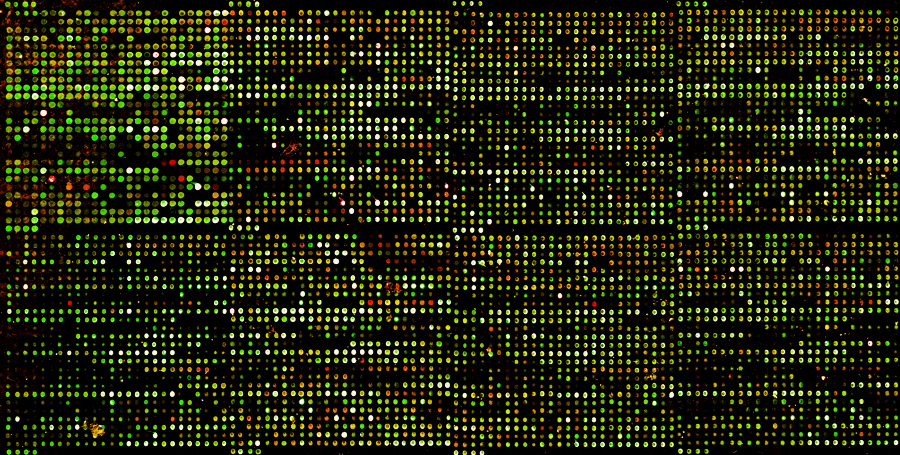
\includegraphics{figs/micro_array.jpg}

}

\caption{Image of a microarray plate,
(http://exploreable.files.wordpress.com/2011/04/array.jpg). Here each
dot is a different variable (different gene) and this image in just one
set of observations that will be placed into a row of the data matrix.}

\end{figure}%

The intuition behind finding these new collective variables rests on the
fact that the original variables have relationships. This is typically
measured using covariance, which quantified how much a pair variables
tends to move in the same direction (positive covariance) or in opposite
directions (negative covariance). If two variables are tighlty coupled,
one can replace the two measurements with one, which will describe how
much the two of them are deviating in some collective way.

It is helpful to think of this geometrically: if the variables are
related, the scatterplot of observed data points will have a shape. The
goal of PCA is to find directions in the \(n\)-dimensional space of
observations that best match the shape of the data cloud. This requires
tools from linear algebra, specifically the technique of change of
basis.

\section{Linearity and vector spaces}\label{linearity-and-vector-spaces}

We have dealt with linear models in various guises, so now would be a
good time to define properly what linearity means. The word comes from
the shape of graphs of linear functions of one variable, e.g.
\(f(x) = a x + b\), but the algebraic meaning rests on the following two
general properties:

\begin{tcolorbox}[enhanced jigsaw, bottomtitle=1mm, coltitle=black, colbacktitle=quarto-callout-note-color!10!white, toprule=.15mm, leftrule=.75mm, titlerule=0mm, breakable, bottomrule=.15mm, arc=.35mm, opacitybacktitle=0.6, opacityback=0, colframe=quarto-callout-note-color-frame, left=2mm, toptitle=1mm, rightrule=.15mm, title=\textcolor{quarto-callout-note-color}{\faInfo}\hspace{0.5em}{Definition}, colback=white]

A \emph{linear transformation} or \emph{linear operator} is a mapping
\(L\) between two sets of vectors with the following properties:

\begin{enumerate}
\def\labelenumi{\arabic{enumi}.}
\tightlist
\item
  \emph{(scalar multiplication)} \(L(c \vec v) = c L(\vec v)\); where
  \(c\) is a scalar and \(\vec v\) is a vector;
\item
  \emph{(additive)}
  \(L(\vec v_1 + \vec v_2) = L(\vec v_1) + L(\vec v_2)\); where
  \(\vec v_1\) and \(\vec v_2\) are vectors.
\end{enumerate}

\end{tcolorbox}

Here we have two types of objects: vectors and transformations/operators
that act on those vectors. The basic example of this are vectors and
matrices, because a matrix multiplied by a vector (on the right) results
another vector, provided the number of columns in the matrix is the same
as the number of rows in the vector. This can be interpreted as the
matrix transforming the vector \(\vec v\) into another one:
\(A \times \vec v = \vec u\).

\textbf{Example:} Let us multiply the following matrix and vector
(specially chosen to make a point):

\begin{Shaded}
\begin{Highlighting}[]
\ImportTok{import}\NormalTok{ numpy }\ImportTok{as}\NormalTok{ np }\CommentTok{\#package for work with arrays and matrices}
\ImportTok{import}\NormalTok{ matplotlib.pyplot }\ImportTok{as}\NormalTok{ plt }\CommentTok{\#package with plotting capabilities}
\ImportTok{import}\NormalTok{ seaborn }\ImportTok{as}\NormalTok{ sns}\OperatorTok{;}\NormalTok{ sns.}\BuiltInTok{set}\NormalTok{() }\CommentTok{\# colors for visualization}
\end{Highlighting}
\end{Shaded}

\begin{Shaded}
\begin{Highlighting}[]
\NormalTok{Mat }\OperatorTok{=}\NormalTok{ np.array([[}\DecValTok{2}\NormalTok{, }\DecValTok{1}\NormalTok{],[}\DecValTok{2}\NormalTok{, }\DecValTok{3}\NormalTok{]])}
\NormalTok{vec1 }\OperatorTok{=}\NormalTok{ np.array([}\DecValTok{1}\NormalTok{, }\OperatorTok{{-}}\DecValTok{1}\NormalTok{])}
\NormalTok{vec2 }\OperatorTok{=}\NormalTok{ Mat}\OperatorTok{@}\NormalTok{vec1}
\BuiltInTok{print}\NormalTok{(vec1)}
\BuiltInTok{print}\NormalTok{(vec2)}
\end{Highlighting}
\end{Shaded}

\begin{verbatim}
[ 1 -1]
[ 1 -1]
\end{verbatim}

We see that this particular vector \((1,-1)\) is unchanged when
multiplied by this matrix, or we can say that the matrix multiplication
is equivalent to multiplication by 1. Here is another such vector for
the same matrix:

\begin{Shaded}
\begin{Highlighting}[]
\NormalTok{vec1 }\OperatorTok{=}\NormalTok{ np.array([}\DecValTok{1}\NormalTok{, }\DecValTok{2}\NormalTok{])}
\NormalTok{vec2 }\OperatorTok{=}\NormalTok{ Mat}\OperatorTok{@}\NormalTok{vec1}
\BuiltInTok{print}\NormalTok{(vec1)}
\BuiltInTok{print}\NormalTok{(vec2)}
\end{Highlighting}
\end{Shaded}

\begin{verbatim}
[1 2]
[4 8]
\end{verbatim}

In this case, the vector is changed, but only by multiplication by a
constant (4). Thus the geometric direction of the vector remained
unchanged.

The notion of linearity leads to the important idea of combining
different vectors:

\begin{tcolorbox}[enhanced jigsaw, bottomtitle=1mm, coltitle=black, colbacktitle=quarto-callout-note-color!10!white, toprule=.15mm, leftrule=.75mm, titlerule=0mm, breakable, bottomrule=.15mm, arc=.35mm, opacitybacktitle=0.6, opacityback=0, colframe=quarto-callout-note-color-frame, left=2mm, toptitle=1mm, rightrule=.15mm, title=\textcolor{quarto-callout-note-color}{\faInfo}\hspace{0.5em}{Definition}, colback=white]

A \emph{linear combination} of \(n\) vectors \(\{ \vec v_i \}\) is a
weighted sum of these vectors with any real numbers \(\{a_i\}\): \[ 
a_1 \vec v_1+ a_2 \vec v_2... + a_n \vec v_n
\]

\end{tcolorbox}

Linear combinations arise naturally from the notion of linearity,
combining the additive property and the scalar multiplication property.
Speaking intuitively, a linear combination of vectors produces a new
vector that is related to the original set. Linear combinations give a
simple way of generating new vectors, and thus invite the following
definition for a collection of vectors closed under linear combinations:

\begin{tcolorbox}[enhanced jigsaw, bottomtitle=1mm, coltitle=black, colbacktitle=quarto-callout-note-color!10!white, toprule=.15mm, leftrule=.75mm, titlerule=0mm, breakable, bottomrule=.15mm, arc=.35mm, opacitybacktitle=0.6, opacityback=0, colframe=quarto-callout-note-color-frame, left=2mm, toptitle=1mm, rightrule=.15mm, title=\textcolor{quarto-callout-note-color}{\faInfo}\hspace{0.5em}{Definition}, colback=white]

A \emph{vector space} is a collection of vectors such that a linear
combination of any \(n\) vectors is contained in the vector space.

\end{tcolorbox}

The most common examples are the spaces of all real-valued vectors of
dimension \(n\), which are denoted by \(\mathbb{R}^n\). For instance,
\(\mathbb{R}^2\) (pronounced ``r two'') is the vector space of two
dimensional real-valued vectors such as \((1,3)\) and
\((\pi, -\sqrt{17})\); similarly, \(\mathbb{R}^3\) is the vector space
consisting of three dimensional real-valued vectors such as
\((0.1,0,-5.6)\). You can convince yourself, by taking linear
combinations of vectors, that these vector spaces contain all the points
in the usual Euclidean plane and three-dimensional space. The real
number line can also be thought of as the vector space \(\mathbb{R}^1\).

\subsection{Linear independence and basis
vectors}\label{linear-independence-and-basis-vectors}

How can we describe a vector space without trying to list all of its
elements? We know that one can generate an element by taking linear
combinations of vectors. It turns out that it is possible to generate
(or ``span'') a vector space by taking linear combinations of a subset
of its vectors. The challenge is to find a minimal subset of subset that
is not redundant. In order to do this, we first introduce a new concept:

\begin{tcolorbox}[enhanced jigsaw, bottomtitle=1mm, coltitle=black, colbacktitle=quarto-callout-note-color!10!white, toprule=.15mm, leftrule=.75mm, titlerule=0mm, breakable, bottomrule=.15mm, arc=.35mm, opacitybacktitle=0.6, opacityback=0, colframe=quarto-callout-note-color-frame, left=2mm, toptitle=1mm, rightrule=.15mm, title=\textcolor{quarto-callout-note-color}{\faInfo}\hspace{0.5em}{Definition}, colback=white]

A set of vectors \(\{ \vec v_i \}\) is called \emph{linearly
independent} if the only linear combination involving them that equals
the zero vector is if all the coefficients are zero. (
\(a_1 \vec v_1 + a_2 \vec v_2 + ... + a_n \vec v_n = 0\) only if
\(a_i = 0\) for all \(i\).)

\end{tcolorbox}

In the familiar Euclidean spaces, e.g.~\(\mathbb{R}^2\), linear
independence has a geometric meaning: two vectors are linearly
independent if the segments from the origin to the endpoint do not lie
on the same line. But it can be shown that any set of three vectors in
the plane is linearly dependent, because there are only two dimensions
in the vector space. This brings us to the key definition of this
section:

\begin{tcolorbox}[enhanced jigsaw, bottomtitle=1mm, coltitle=black, colbacktitle=quarto-callout-note-color!10!white, toprule=.15mm, leftrule=.75mm, titlerule=0mm, breakable, bottomrule=.15mm, arc=.35mm, opacitybacktitle=0.6, opacityback=0, colframe=quarto-callout-note-color-frame, left=2mm, toptitle=1mm, rightrule=.15mm, title=\textcolor{quarto-callout-note-color}{\faInfo}\hspace{0.5em}{Definition}, colback=white]

A \emph{basis} of a vector space is a linearly independent set of
vectors that generate (or span) the vector space. The number of vectors
(cardinality) in such a set is called the \emph{dimension} of the vector
space.

\end{tcolorbox}

A vector space generally has many possible bases, as illustrated in
figure. In the case of \(\mathbb{R}^2\), the usual (canonical) basis set
is \(\{(1,0); (0,1)\}\) which obviously generates any point on the plane
and is linearly independent. But any two linearly independent vectors
can generate any vector in the plane.

\textbf{Example:} The vector \(\vec r = (2,1)\) can be represented as a
linear combination of the two canonical vectors:
\(\vec r = 2\times (1,0)+1\times (0,1)\). Let us choose another basis
set, say \(\{(1,1); (-1,1)\}\) (this is the canonical basis vectors
rotated by \(\pi/2\).) The same vector can be represented by a linear
combination of these two vectors, with coefficients \(1.5\) and
\(-0.5\): \(\vec r = 1.5\times (1,1) - 0.5 \times (-1,1)\). If we call
the first basis \(C\) for canonical and the second basis \(D\) for
different, we can write the same vector using different sets of
coordinates for each basis:

\[ 
\vec r_{C} = (2,1); \; \vec r_D = (1.5, -0.5)
\]

\subsection{Projections and changes of
basis}\label{projections-and-changes-of-basis}

The representation of an arbitrary vector (point) in a vector space as a
linear combination of a given basis set is called the
\emph{decomposition} of the point in terms of the basis, which gives the
coordinates for the vector in terms of each basis vector. The
decomposition of a point in terms of a particular basis is very useful
in high-dimensional spaces, where a clever choice of a basis can allow a
description of a set of points (such as a data set) in terms of
contributions of only a few basis vectors, if the data set primarily
extends only in a few dimensions.

To obtain the coefficients of the basis vectors in a decomposition of a
vector \(\vec r\), we need to perform what is termed a \emph{projection}
of the vector onto the basis vectors. Think of shining a light
perpendicular to the basis vector, and measuring the length of the
shadow cast by the vector \(\vec r\) onto \(\vec v_i\). If the vectors
are parallel, the shadow is equal to the length of \(\vec r\); if they
are orthogonal, the shadow is nonexistent. To find the length of the
shadow, use the inner product of \(\vec r\) and \(\vec v\), which as you
recall corresponds to the cosine of the angle between the two vectors
multiplied by their norms:
\(\left \langle \vec r, \vec v\right \rangle =\vert\vec r\vert \vert\vec v\vert\cos(\theta)\).
We do not care about the length of the vector \(\vec v\) we are
projecting onto, thus we divide the inner product by the square norm of
\(\vec v\), and then multiply the vector \(\vec v\) by this projection
coefficient:

\[ 
Proj(\vec r ; \vec v) = \frac{ \langle \vec r , \vec v \rangle  } {\langle \vec v , \vec v \rangle } \vec v = \frac{ \langle \vec r ,  \vec v \rangle  } {\vert \vec v \vert^2} \vec v= \frac{  \vert\vec r\vert \cos(\theta) } {\vert \vec v \vert}\vec v
\]

This formula gives the projection of the vector \(\vec r\) onto
\(\vec v\), the result is a new vector in the direction of \(\vec v\),
with the scalar coefficient
\(a = \langle \vec r ,\vec v \rangle /\vert \vec v \vert^2\).

\textbf{Example:} Here is how one might calculate the projection of the
point \((2,1)\) onto the basis set \(\{(1,1); (-1,1)\}\):

\begin{Shaded}
\begin{Highlighting}[]
\NormalTok{v1 }\OperatorTok{=}\NormalTok{ np.array([}\DecValTok{1}\NormalTok{, }\DecValTok{1}\NormalTok{]) }\CommentTok{\# basis vector 1}
\NormalTok{v2 }\OperatorTok{=}\NormalTok{ np.array([}\OperatorTok{{-}}\DecValTok{1}\NormalTok{, }\DecValTok{1}\NormalTok{]) }\CommentTok{\# basis vector 2}
\NormalTok{u }\OperatorTok{=}\NormalTok{ np.array([}\DecValTok{2}\NormalTok{, }\DecValTok{1}\NormalTok{])  }\CommentTok{\# a vector represented in usual coordinates}
\NormalTok{ProjMat }\OperatorTok{=}\NormalTok{ np.array([[v1], [v2]]) }\CommentTok{\# matrix of basis vectors}
\BuiltInTok{print}\NormalTok{(ProjMat) }\CommentTok{\# print the matrix}
\BuiltInTok{print}\NormalTok{(ProjMat}\OperatorTok{@}\NormalTok{u) }\CommentTok{\# print the coordinates in the new basis}
\end{Highlighting}
\end{Shaded}

\begin{verbatim}
[[[ 1  1]]

 [[-1  1]]]
[[ 3]
 [-1]]
\end{verbatim}

This is not quite right: the projection coefficients are off by a factor
of two compared to the correct values in the example above. This is
because we have neglected to \emph{normalize} the basis vectors, so we
should modify the script as follows:

\begin{Shaded}
\begin{Highlighting}[]
\NormalTok{v1 }\OperatorTok{=}\NormalTok{ v1}\OperatorTok{/}\NormalTok{np.}\BuiltInTok{sum}\NormalTok{(v1}\OperatorTok{**}\DecValTok{2}\NormalTok{) }\CommentTok{\# normalize basis vector 1}
\NormalTok{v2 }\OperatorTok{=}\NormalTok{ v2}\OperatorTok{/}\NormalTok{np.}\BuiltInTok{sum}\NormalTok{(v2}\OperatorTok{**}\DecValTok{2}\NormalTok{) }\CommentTok{\# normalize basis vector 2}
\NormalTok{ProjMat }\OperatorTok{=}\NormalTok{ np.array([[v1], [v2]]) }\CommentTok{\# matrix of basis vectors}
\BuiltInTok{print}\NormalTok{(ProjMat) }\CommentTok{\# print the matrix}
\BuiltInTok{print}\NormalTok{(ProjMat}\OperatorTok{@}\NormalTok{u) }\CommentTok{\# print the coordinates in the new basis}
\end{Highlighting}
\end{Shaded}

\begin{verbatim}
[[[ 0.5  0.5]]

 [[-0.5  0.5]]]
[[ 1.5]
 [-0.5]]
\end{verbatim}

This is an example of how to convert a vector/point from representation
in one basis set to another. The new basis vectors, expressed in the
original basis set, are arranged in a matrix by row, scaled by their
norm squared, and multiplied by the vector that one wants to express in
the new basis. The resulting vector contains the coordinates in the new
basis.

\section{PCA algorithm}\label{pca-algorithm}

We start with a data set \(X\) in the form of a \(m\) by \(n\) matrix.
The first step is to decide which are the variables and which are the
observations. For example, in the case of the microarray experiment, it
usually makes sense to consider different genes the variables, and to
use principal components to see which genes tend to be expressed
together with others.

The second step is to compute the variance-covariance matrix of the
\(N\) variables.

\begin{tcolorbox}[enhanced jigsaw, bottomtitle=1mm, coltitle=black, colbacktitle=quarto-callout-note-color!10!white, toprule=.15mm, leftrule=.75mm, titlerule=0mm, breakable, bottomrule=.15mm, arc=.35mm, opacitybacktitle=0.6, opacityback=0, colframe=quarto-callout-note-color-frame, left=2mm, toptitle=1mm, rightrule=.15mm, title=\textcolor{quarto-callout-note-color}{\faInfo}\hspace{0.5em}{Definition}, colback=white]

The \emph{variance-covariance} matrix \(C\) of a data set \(X\) with
\(n\) variables \(x_i\) and \(m\) observations is an \(n\) by \(n\)
matrix that contains pairwise variances between all \(n\) variables, so
that its \(i\), \(j\) element is:

\[C_{i,j} = Cov(X_i,X_j)\]

\end{tcolorbox}

The third step is to diagonalize (find the eigenvalues and eigenvectors)
of the covariance matrix \(C\). The eigenvectors are the principal
components of the \(n\) variables in the data set, representing linear
combinations of the variables that best fit the data. Diagonalizing an
\(n\) by \(n\) matrix results in \(n\) eigenvectors, so in order to
simplify the description one needs to choose the most significant ones.
This is accomplished by choosing a subset of \(k\) principal components
with the largest eigenvalues. Here are the steps of principal component
analysis (PCA):

\begin{tcolorbox}[enhanced jigsaw, bottomtitle=1mm, coltitle=black, colbacktitle=quarto-callout-tip-color!10!white, toprule=.15mm, leftrule=.75mm, titlerule=0mm, breakable, bottomrule=.15mm, arc=.35mm, opacitybacktitle=0.6, opacityback=0, colframe=quarto-callout-tip-color-frame, left=2mm, toptitle=1mm, rightrule=.15mm, title=\textcolor{quarto-callout-tip-color}{\faLightbulb}\hspace{0.5em}{PCA algorithm}, colback=white]

\begin{enumerate}
\def\labelenumi{\arabic{enumi}.}
\tightlist
\item
  Obtain a dataset as a \(m\) by \(n\) matrix, with \(n\) variables and
  \(m\) observations
\item
  Compute covariances for variable i and variable j, put them in the
  covariance matrix \(C\)
\item
  Compute the eigenvalues and eigenvectors (principal components) of the
  matrix \(C\)
\item
  Order the principal component by size of eigenvalues from largest to
  smallest and select a few as the new coordinates
\end{enumerate}

\end{tcolorbox}

\section{Optimization by explained
variance}\label{optimization-by-explained-variance}

The reason that we order the PCs by their eigenvalues is that they
measure the amount of variance captured by each principal component. In
that, they are equivalent to the coefficient of determination \(r^2\) in
linear regression. The sum of all the eigenvalues is equal to the total
variance of all the variables:

\[ 
\sum_i \lambda_i = \sum Var(X_i)
\]

and the fraction of variance captured by the a principal component is:

\[ Var(PC_i) = \frac{\lambda_i}{\sum_i \lambda_i}\]

The theory behind this rests on some relatively sophisticated linear
algebra, in particular what is called the singular value decomposition
(SVD) and the Eckart-Young Mirsky theorem. Here is a nice video by
Gilbert Strang that explains
this:\href{https://www.youtube.com/watch?v=Y4f7K9XF04k}{Strang lecture}

\section{Dimensionality reduction}\label{dimensionality-reduction}

After sorting the principal components and selecting \(k\) largest
eigenvalues, we are ready to simplify the data. This means that we can
express a data set of \(n\) variables in terms of the coordinate set of
\(k\) principal components. In order to express the data set in this new
system of coordinates, we compute the projection coefficients for each
measurement onto a give principal component. Suppose that \(Y\) is a set
of measurements of \(N\) variables (e.g.~genes) and \(P_i\) is the
\(i\)-the principal component. Then the projection coefficient of \(Y\)
onto \(P_i\) is the dot product of the two vectors (both of length
\(N\)) divided by the squared norm (length) of the PC:

\[ c_i = \frac{\langle Y, P_i\rangle}{|| P_i ||^2} \]

If the eigenvectors are normalized prior to the computation (as they are
by most computational packages), then the projection coefficient is just
the dot product. Then the coefficients can be obtained for all of the
measurements in the data set \(X\) (\(m\) by \(n\)) by multiplying it by
the matrix \(P\) containing the first \(k\) eigenvectors (principal
components), which has \(n\) rows and \(k\) columns. The result is an
\(m\) by \(k\) matrix \(C\) containing \(k\) coefficients for each of
the \(m\) measurements:

\[
C = D \times P
\]

Here is the outline for the transformation:

\begin{tcolorbox}[enhanced jigsaw, bottomtitle=1mm, coltitle=black, colbacktitle=quarto-callout-tip-color!10!white, toprule=.15mm, leftrule=.75mm, titlerule=0mm, breakable, bottomrule=.15mm, arc=.35mm, opacitybacktitle=0.6, opacityback=0, colframe=quarto-callout-tip-color-frame, left=2mm, toptitle=1mm, rightrule=.15mm, title=\textcolor{quarto-callout-tip-color}{\faLightbulb}\hspace{0.5em}{Dimensionality reduction}, colback=white]

\begin{enumerate}
\def\labelenumi{\arabic{enumi}.}
\tightlist
\item
  Subtract the mean of each observation from the data matrix (if it has
  \(M\) observations in rows and \(N\) variables as columns, subtract
  the mean of each row from it)
\item
  Compute the projection coefficients \(C = D \times P\) for each
  measurement and each of the \(k\) principal components
\item
  Plot or otherwise display these coefficients as coordinates in the new
  vector system of the \(k\) PCs. This can be used to cluster or
  otherwise find patterns in the observations.
\end{enumerate}

\end{tcolorbox}

The entire data set can be expressed in a low-dimensional setting, for
instance plotted in the plane of two principal components with
coordinates \((c_{i,1}, c_{i,2})\) for each data measurement \(i\). This
is often useful for clustering, or grouping experimental conditions
based on the similarity of their principal component representations.
Biologists frequently do this with complex data sets, for example
grouping different cell lines together by their gene expression
profiles.

\bookmarksetup{startatroot}

\chapter{Optimization using
gradients}\label{optimization-using-gradients}

\section{Overview}\label{overview}

One often has to find the maximum or minimum of a function that
describes an important biological property. Examples include:

\begin{itemize}
\item
  Free energy of a protein as function of its conformation (the folding
  problem)
\item
  Evolutionary fitness as a function of the genome
\item
  Optimizing the dose of therapeutic radiation or chemotherapy, to
  affect the maximal fraction of tumor cells and the minimal number of
  healthy cells
\end{itemize}

In all these cases, there is the same fundamental problem: given a
complex function of many variables, find the values of the variables
which optimize the function, that is, for which it attains its maximum
or minimum, depending on the question.

Some terminology: \(f\) is known as the \emph{objective function}, and
the quantities the function depends on (\(x_1, x_2, ..., x_n\)) are the
governing variables.

It is important to note the notion of a minimum or a maximum is local:
it is a point which is lowest or highest in some neighborhood. But very
often we are interested in a global optimum - the best possible solution
to our problem. The first problem is not too difficult, while the second
is practically impossible for a complex function, because, aside from
the areas explored by minimization, there is no way to guarantee that
there is no better optimum elsewhere. This is the tragic state of
optimizers everywhere - they have to live with the uncertainty.

\section{Optimization with one
variable}\label{optimization-with-one-variable}

\subsection{golden section search}\label{golden-section-search}

Let us first consider searching for the minimum (or maximum, the
problems are really the same except for a minus sign) of a function of
one variable \(f(x)\). The goal is to locate the minimum value of the
function within a certain interval on the \(x\)-axis, to a desired
tolerance. We assume only that we can evaluate the function at any given
value of \(x\). Here is the outline of the algorithm:

\begin{tcolorbox}[enhanced jigsaw, bottomtitle=1mm, coltitle=black, colbacktitle=quarto-callout-note-color!10!white, toprule=.15mm, leftrule=.75mm, titlerule=0mm, breakable, bottomrule=.15mm, arc=.35mm, opacitybacktitle=0.6, opacityback=0, colframe=quarto-callout-note-color-frame, left=2mm, toptitle=1mm, rightrule=.15mm, title=\textcolor{quarto-callout-note-color}{\faInfo}\hspace{0.5em}{Golden section search}, colback=white]

\begin{enumerate}
\def\labelenumi{\arabic{enumi}.}
\tightlist
\item
  start with three points \(x_1,x_2,x_3\) \((x_1<x_2<x_3)\), such that
  \(f(x_2) < f(x_1)\) and \(f(x_2) < f(x_3)\)
\item
  choose a point \(x_4\) in the larger of the intervals \((x_1,x_2)\) or
  \((x_2,x_3)\) (let's assume it's \((x_1,x_2)\), the process is the
  same for the other case)
\item
  if \(f(x_4) > f(x_2)\), replace \(x_1\) with \(x_4\), the new triplet
  is \((x_4, x_2, x_3)\)
\item
  if \(f(x_4) < f(x_2)\), replace \(x_3\) with \(x_2\), the new triplet
  is \((x_1, x_4, x_2)\)
\item
  repeat until the width of the interval is smaller than your tolerance
\end{enumerate}

\end{tcolorbox}

\begin{figure}[H]

{\centering 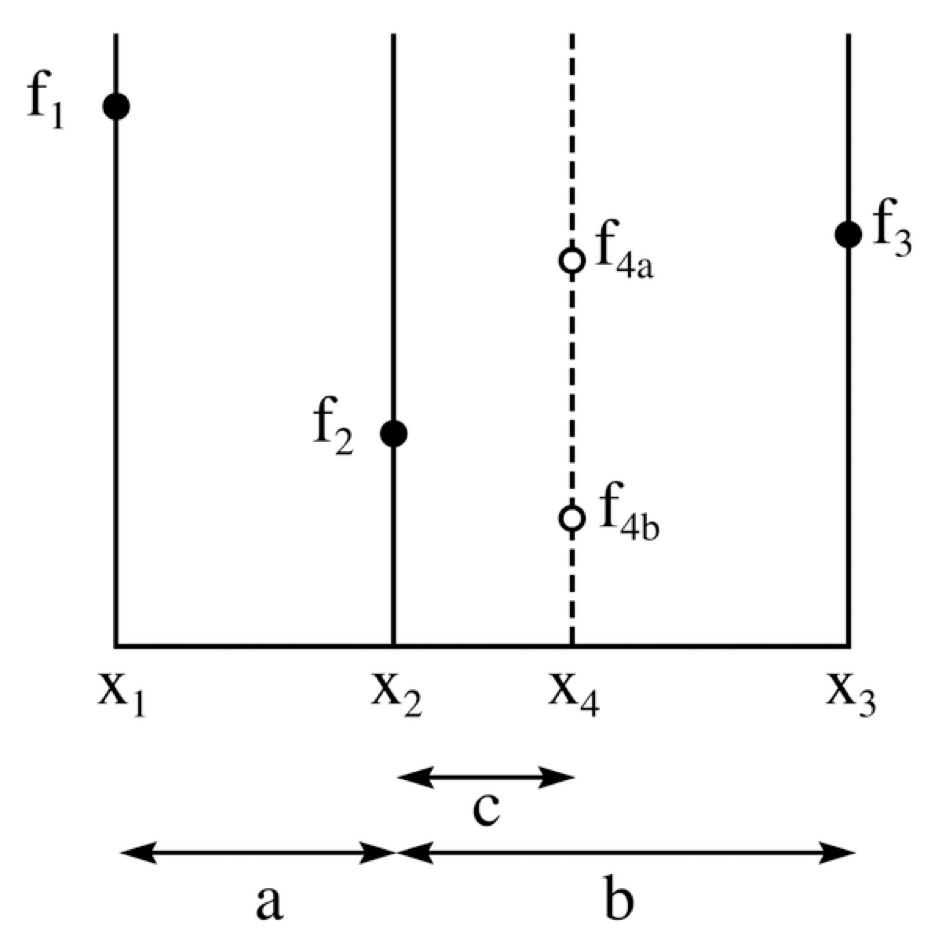
\includegraphics{figs/golden_search.png}

}

\caption{Golden ratio method for a 1-variable function f(x);
\href{https://en.wikipedia.org/wiki/Golden-section_search\#/media/File:GoldenSectionSearch.png}{Figure
source}}

\end{figure}%

The question is, what is the optimal way to pick the new point \(x_4\)?
Since we have no information about the shape of the function \(f(x)\),
we don't know where the minimum is more likely to be hiding. The best
approach is to hedge your bets and make each option (3 or 4) result in
the same interval scaled by the same factor.

Assume that we pick \(x_4\) in \((x_1, x_2)\), as the larger interval,
and we want to pick \(x_4\) so that the length is reduced by the same
factor in both cases: \((x_4, x_2, x_3)\) and \((x_1, x_4, x_2)\) and
the resulting triplet is also divided in the same proportion. This is
the condition for the golden ratio (that the ratio of the larger segment
to the whole is the same as the ratio of the smaller segment to the
larger). Thus, the the choice for the new point is
\(x_4 = x_1 + (x_3 - x_1)/\phi\), where \(\phi = (1 + \sqrt 5)/2\).
Similarly, if the interval \((x_2,x_3)\) is larger, we pick
\(x_4 = x_3 - (x_3 - x_1)/\phi\).

Notice that this means that the interval bracketing the minimum shrinks
by a factor of \(\phi \approx 1.61\) every step.

\subsection{bisection method}\label{bisection-method}

The bisection method is applicable for a continuous function \(f(x)\)
which has a computable derivative function \(F(x)\). In that case,
finding a maximum or minimum of f(x) is the same as finding a root of
the derivative function F(x). The bisection method simply divides the
bracketing interval that contains the maximum or minimum into two, like
this:

\begin{figure}[H]

{\centering 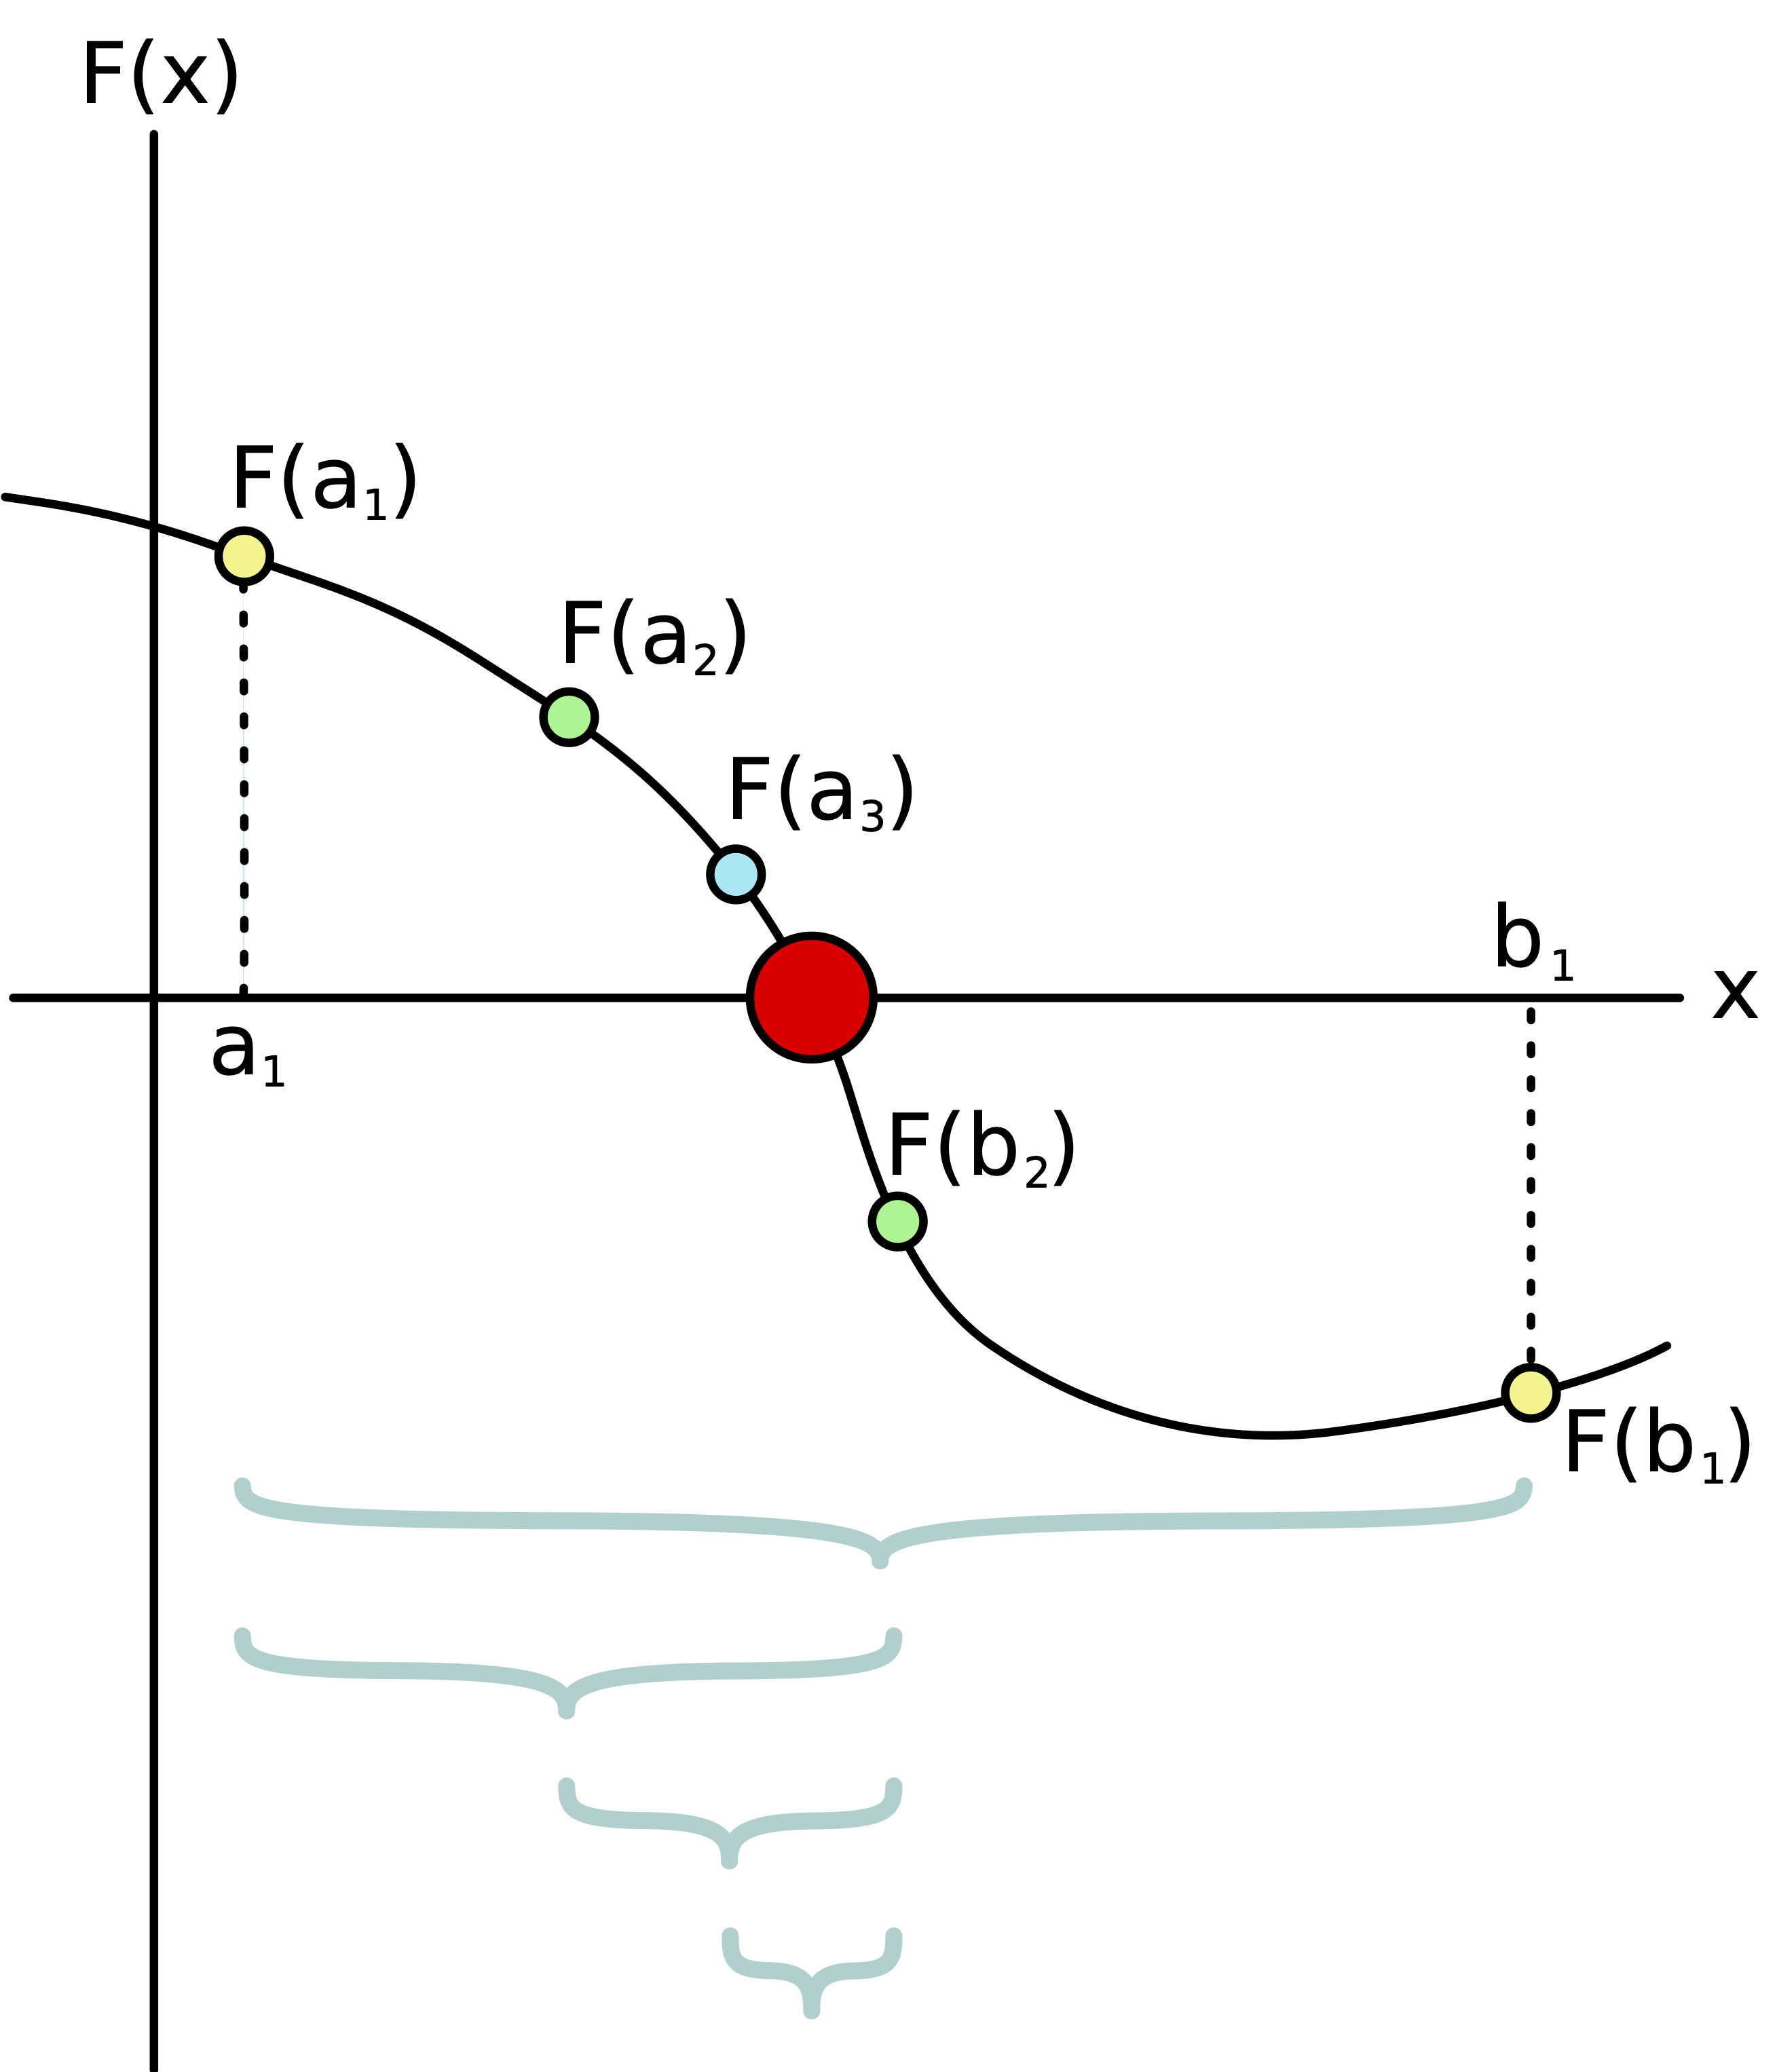
\includegraphics{figs/Bisection_method.png}

}

\caption{Bisection method involves cutting the interval bracketing a
zero in two;
\href{https://en.wikipedia.org/wiki/Bisection_method\#/media/File:Bisection_method.svg}{Figure
source}}

\end{figure}%

\begin{tcolorbox}[enhanced jigsaw, bottomtitle=1mm, coltitle=black, colbacktitle=quarto-callout-note-color!10!white, toprule=.15mm, leftrule=.75mm, titlerule=0mm, breakable, bottomrule=.15mm, arc=.35mm, opacitybacktitle=0.6, opacityback=0, colframe=quarto-callout-note-color-frame, left=2mm, toptitle=1mm, rightrule=.15mm, title=\textcolor{quarto-callout-note-color}{\faInfo}\hspace{0.5em}{Golden section search}, colback=white]

\begin{enumerate}
\def\labelenumi{\arabic{enumi}.}
\tightlist
\item
  start with an interval \((a,b)\) with \(F(a)\) and \(F(b)\) of
  opposite signs
\item
  choose \(c = (b-a)/2\)
\item
  pick the side on which the two endpoints are bracketing zero, so the
  new interval is either \((a,c)\) or \((c,b)\)
\item
  repeat until the interval width is smaller than the tolerance
\end{enumerate}

\end{tcolorbox}

In this case, the bracketing interval is always decreased by a factor of
two, which is faster than the golden section search.

\subsection{secant method}\label{secant-method}

Secant method is also a root-finding method, and can thus be used to
find optima of functions with a computable derivative. If the derivative
function is f(x), then the algorithm is:

\begin{tcolorbox}[enhanced jigsaw, bottomtitle=1mm, coltitle=black, colbacktitle=quarto-callout-note-color!10!white, toprule=.15mm, leftrule=.75mm, titlerule=0mm, breakable, bottomrule=.15mm, arc=.35mm, opacitybacktitle=0.6, opacityback=0, colframe=quarto-callout-note-color-frame, left=2mm, toptitle=1mm, rightrule=.15mm, title=\textcolor{quarto-callout-note-color}{\faInfo}\hspace{0.5em}{Secant algorithm}, colback=white]

\begin{enumerate}
\def\labelenumi{\arabic{enumi}.}
\tightlist
\item
  start with a bracketing interval \((x_0, x_1)\)
\item
  calculate the slope of the (secant) line that connects the two points
  \(a = \frac{f(x_1) - f(x_0)}{x_1 - x_0}\)
\item
  pick the next value \(x_i = x_{i-1} - af(x_{i-1})\), which is where
  the secant line crosses 0
\item
  repeat until \(f(x_i)\) is close enough to zero
\end{enumerate}

\end{tcolorbox}

\begin{figure}[H]

{\centering 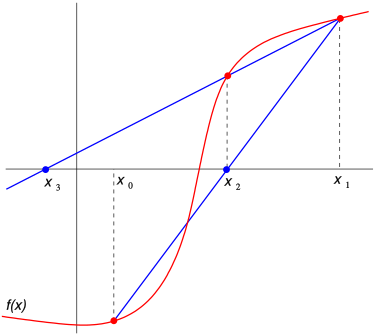
\includegraphics{figs/Secant_method.png}

}

\caption{The secant method uses the line connecting the two bracketing
points to approximate the root;
\href{https://commons.wikimedia.org/w/index.php?curid=877497}{Figure
source}}

\end{figure}%

The secant method is faster to converge than bisection for most
functions.

\subsection{Newton-Raphson method}\label{newton-raphson-method}

We will now consider an old method for finding roots of functions,
devised by the Great Newton Himself, is also useful for finding maxima
and minima of functions for which an exact formula is given. To use for
optimization, it requires not only the knowledge of the derivative
function \(f(x)\) (as for secant and bisection method) but also the
knowledge of the second derivative function \(f'(x)\) of the function we
want to optimize.

The idea is based on the first-order Taylor expansion of a function near
a point \(x_0\):
\(f(x_0 + \Delta x) = f(x_0) + \Delta x f'(x_0) + ...\). The dots
indicate higher-order terms that we will ignore, for sufficiently small
\(\Delta x\). Now, suppose the function has a root (zero) at \(x_0\), so
\(f(x_0) = 0\). Then, if we are at a point near the root,
\(x_0 + \Delta x\), we can calculate how far away it is from the root,
by simply solving for \(\Delta x = f(x_0 + \Delta x) / f'(x_0)\). The
idea of Newton's method is to find the step size needed to reach the
root, by using the value of the derivative at the current point
\(x_0 + \Delta x\) (assuming the points are close enough that the slopes
are almost equal). Then the steps for the algorithm are:

\begin{tcolorbox}[enhanced jigsaw, bottomtitle=1mm, coltitle=black, colbacktitle=quarto-callout-note-color!10!white, toprule=.15mm, leftrule=.75mm, titlerule=0mm, breakable, bottomrule=.15mm, arc=.35mm, opacitybacktitle=0.6, opacityback=0, colframe=quarto-callout-note-color-frame, left=2mm, toptitle=1mm, rightrule=.15mm, title=\textcolor{quarto-callout-note-color}{\faInfo}\hspace{0.5em}{Newton-Raphson algorithm in 1 dimension}, colback=white]

\begin{enumerate}
\def\labelenumi{\arabic{enumi}.}
\item
  Start at some point \(x_0\) (not the root, as above)
\item
  Let \(x_{i+1} = x_i - f(x_i)/f'(x_i)\)
\item
  Repeat, until \(|x_{i+1} - x_i|< \epsilon_{tol}\), where
  \(\epsilon_{tol}\) is the specified tolerance
\end{enumerate}

\end{tcolorbox}

\begin{figure}[H]

{\centering 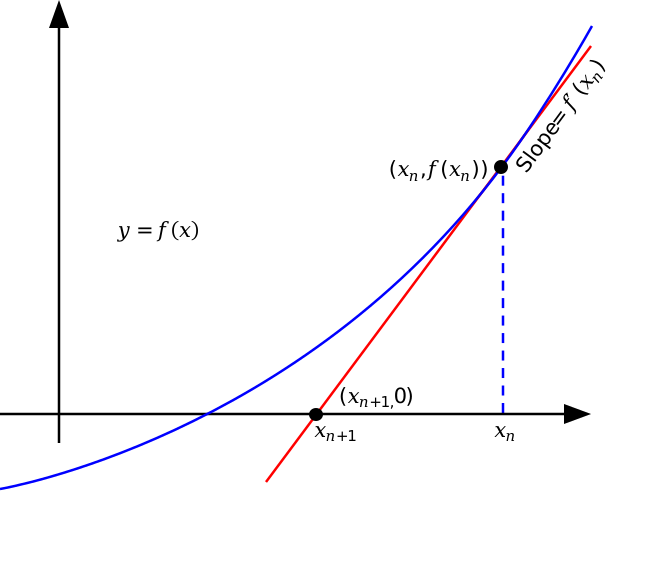
\includegraphics{figs/Newton_iteration.png}

}

\caption{Newton-Raphson method for finding roots uses the derivative of
the function to find the intersection of the tangent line with the
x-axis;
\href{https://commons.wikimedia.org/wiki/File:Newton_iteration.svg}{Figure
source}}

\end{figure}%

The method turns out to be very efficient. Its only limitation is that
it cannot find a root for which the derivative is zero (graphically, a
root at which the graph of the function only touches the \(x\)-axis).
Another complication is that, if the starting point is not close enough
to a root, it can be hard to predict which root the method will find,
but once it settles in near one, it will reach it quickly. If the value
of the derivative \(f'(x_i)\) is small, then the method can bounce
around, sometimes almost chaotically, so its efficiency strongly depends
on starting in proximity to a root.

To be used for optimization of a function \(F(x)\), we need to be able
to calculate \(F'(x) = f(x)\) and \(F''(x) = f'(x)\) and the find the
root(s) of \(f(x)\). Then one has to check whether the extremum is a max
or a min, which is straightforward.

\section{Optimization of multivariable functions using
derivatives}\label{optimization-of-multivariable-functions-using-derivatives}

Let us now consider functions of multiple variables, which is the case
for most real applications. Such, a function, e.g.~\(f(x,y)\), takes in
values of the variables \(x\) and \(y\), and returns a single number.
Graphically, this could be plotted as a surface, with the height at any
pair of coordinates \((x,y)\) given by \(f(x,y)\). Intuitively, the goal
of optimization is to find the lowest (or highest) point on the surface,
at least in a neighborhood (see above discussion about difficulties of
global optimization). Let us assume that we are searching for a minimum,
as the story is completely equivalent for maximization.

\subsection{multivariable optimization
problem}\label{multivariable-optimization-problem}

A function of more than one variable is denoted by \(f(\vec x)\), where
\(\vec x\) is a vector of \(n\) variables \(x_1, x_2, ..., x_n\). This
means the function takes in a vector of several numbers and returns a
scalar - a single number. One simple visual analogy is the function that
gives elevation (height) for a given latitude and longitude \((x,y)\).
By plotting that function we would produce the shape of a mountain range
or any other terrain, with the appropriate height at each point in the
\(x-y\) plane.

The basic condition for finding the maximum or minimum of a function is
known from basic calculus. For a function of \(n\) variables
\(f(x_1, x_2, ..., x_n)\) to be at an optimum, all partial derivatives
must vanish:

\[ \frac{\partial f(x_1, x_2, ..., x_n)}{\partial x_1} = \frac{\partial f(x_1, x_2, ..., x_n)}{\partial x_2} = ... = \frac{\partial f(x_1, x_2, ..., x_n)}{\partial x_n} = 0 \]

This gives a set of \(n\) equations to be solved for \(n\) unknowns.
However, in practice optimization problems are rarely solved this way,
because solving \(n\) nonlinear equations can be difficult, particularly
for complicated functions that frequently arise in biology. However, one
can use iterative methods to converge to the optimum using derivatives
of the objective function.

\subsection{gradient and contours}\label{gradient-and-contours}

In order to describe the changes in multivariable functions, we need
more than one number. Consider the slope on the surface of a mountain:
it may be steep in one direction, and flat in another. In order to deal
with this, \emph{partial derivatives} are used. These represent the rate
of change of \(f\) with respect to \(x\) and \(y\) separately.
Geometrically, this means the slope of the landscape we visualized
above, if sliced in the \(x\) or \(y\) direction.

\textbf{Example:} If \(f(x,y) = x^2-2x+y^2+4x+5\)

\[
\frac{\partial f}{\partial x} = 2x -2 \\
\frac{\partial f}{\partial y} = 2y +4 
\]

This allows us to define the multi-dimensional equivalent of the
derivative: the \emph{gradient} of a function,

\begin{tcolorbox}[enhanced jigsaw, bottomtitle=1mm, coltitle=black, colbacktitle=quarto-callout-note-color!10!white, toprule=.15mm, leftrule=.75mm, titlerule=0mm, breakable, bottomrule=.15mm, arc=.35mm, opacitybacktitle=0.6, opacityback=0, colframe=quarto-callout-note-color-frame, left=2mm, toptitle=1mm, rightrule=.15mm, title=\textcolor{quarto-callout-note-color}{\faInfo}\hspace{0.5em}{Definition}, colback=white]

The \emph{gradient} of a function \(f(\vec x)\) of multiple variables
\(\vec x = x_1, .., x_n\) is a vector with \(n\) components, each one
the partial derivative with respect to the corresponding variable:

\[ \nabla f (\vec x) = (\frac{\partial f}{\partial x_1}, \frac{\partial f}{\partial x_2}, ..., \frac{\partial f}{\partial x_n}) \]

\end{tcolorbox}

To gain some geometric intuition about gradients, let us introduce the
notion of contours of \(f(\vec x)\)

\begin{tcolorbox}[enhanced jigsaw, bottomtitle=1mm, coltitle=black, colbacktitle=quarto-callout-note-color!10!white, toprule=.15mm, leftrule=.75mm, titlerule=0mm, breakable, bottomrule=.15mm, arc=.35mm, opacitybacktitle=0.6, opacityback=0, colframe=quarto-callout-note-color-frame, left=2mm, toptitle=1mm, rightrule=.15mm, title=\textcolor{quarto-callout-note-color}{\faInfo}\hspace{0.5em}{Definition}, colback=white]

The \emph{contours} or \emph{level curves} of a function \(f(\vec x)\)
of multiple variables \(\vec x = x_1, .., x_n\) are sets of values of
\(\vec x\) that satisfy equations, for any given constant c:

\[ f (\vec x) = c \]

\end{tcolorbox}

These are curves (for two-variable functions) or surfaces (for
three-variable functions) in the space of the variables on which the
function is equal to a particular constant. One common example of this
are contours of a landscape (e.g.~on the Earth's surface) on a
topographical map.

There is an important relationship between gradients and contours. Since
there there is no change in \(f\) as one travels along it, the
derivative of the function in the direction of the contour curve at any
point is 0. As a consequence, the direction of the fastest change of
\(f\) at any point, \(\nabla f\) is orthogonal to the level curve at
that point.

\textbf{Example:} Let us find the contours (level curves) for the
function we gave above, which means the solution of the equation
\(f(x,y) = (x-1)^2+(y+2)^2 = c\). These are circles centered at
\((1,-2)\), with the radius depending on the value of \(c\).

Let us compare the direction of the gradient at a point, let us say at
\((0,-2)\). This point is horizontally to the left of the center of the
circular level curves. Thus, the tangent line to the circle at the point
is vertical. The gradient is \(\nabla f = (-2,0)\): a vertical vector,
perpendicular to the direction of the circle at that point.

\subsection{gradient descent}\label{gradient-descent}

The simplest idea for finding the lowest point in a valley is to follow
the slope downward. In multiple dimensions, the direction of greatest
downward change (steepest descent) is given by the gradient, which leads
to the \emph{gradient descent} algorithm.

The first method for minimization of a multidimensional function simply
takes steps in the direction of the gradient, until the point is
sufficiently close to the bottom of the valley. This is called the
method of \emph{gradient descent}:

\begin{tcolorbox}[enhanced jigsaw, bottomtitle=1mm, coltitle=black, colbacktitle=quarto-callout-note-color!10!white, toprule=.15mm, leftrule=.75mm, titlerule=0mm, breakable, bottomrule=.15mm, arc=.35mm, opacitybacktitle=0.6, opacityback=0, colframe=quarto-callout-note-color-frame, left=2mm, toptitle=1mm, rightrule=.15mm, title=\textcolor{quarto-callout-note-color}{\faInfo}\hspace{0.5em}{Gradient descent algorithm}, colback=white]

\begin{enumerate}
\def\labelenumi{\arabic{enumi}.}
\item
  Start at some point \(\vec x_0\).
\item
  Compute the gradient at the current point \(\vec x_i\),
  \(\nabla f (\vec x_i)\). Find the minimum of the function \(f\) along
  that direction, which may be done through a one-dimensional search.
\item
  Take the next point to be
  \(x_{i+1} = x_i + \alpha \nabla f (\vec x_i)\), where \(\alpha\) is
  the multiple found by the one-dimensional search.
\item
  Repeat until \(|| \vec x_{i+1} - \vec x_i || < \epsilon_{tol}\), where
  \(\epsilon_{tol}\) is the specified tolerance.
\end{enumerate}

\end{tcolorbox}

The gradient descent method, although intuitively simple, is in practice
inefficient. Specifically, it has difficulties with descending into a
long, narrow valley: it takes many short, zigzagging steps on the way to
the lowest point. Relying on the steepest way down is not the fastest
way of reaching the minimum, although it is guaranteed to converge
eventually, if it takes small steps.

\subsection{Newton-Raphson method}\label{newton-raphson-method-1}

A different approach at finding the minimum of a multi-variable function
is to extend the Newton-Raphson method from one variable to multiple.
The idea is once again to convert the optimization problem for
\(f(\vec x)\) into a root-finding problem for \(\nabla f (\vec x)\)
where the gradient function plays the role of the derivative in the
1-dimensional Newton's method. In order for this to work, we need an
equivalent to the second derivative as well.

\begin{tcolorbox}[enhanced jigsaw, bottomtitle=1mm, coltitle=black, colbacktitle=quarto-callout-note-color!10!white, toprule=.15mm, leftrule=.75mm, titlerule=0mm, breakable, bottomrule=.15mm, arc=.35mm, opacitybacktitle=0.6, opacityback=0, colframe=quarto-callout-note-color-frame, left=2mm, toptitle=1mm, rightrule=.15mm, title=\textcolor{quarto-callout-note-color}{\faInfo}\hspace{0.5em}{Definition}, colback=white]

For a function \(f(\vec x)\) of a vector variable \(\vec x\) with \(n\)
components, the \emph{Hessian} is a \(n\) by \(n\) matrix, with each
element defined as the second partial with respect to two variables:

\[ 
H_{i,j} = \frac{\partial^2 f}{\partial x_i \partial x_j} 
\]

\end{tcolorbox}

\textbf{Example:} For the same function we saw
\(f(x,y) = x^2-2x+y^2+4x+5\), with the gradient:

\[
\frac{\partial f}{\partial x} = 2x -2 \\
\frac{\partial f}{\partial y} = 2y +4 
\]

The Hessian requires computing two more partials for each of the
elements of the gradient:

\[
\frac{\partial^2 f}{\partial x^2} = 2 \\
\frac{\partial^2 f}{\partial x \partial y} = 0 \\
\frac{\partial^2 f}{\partial y \partial x} = 0 \\
\frac{\partial^2 f}{\partial y^2} = 2
\]

So the Hessian matrix is

\[
H(f(\vec x)) = \begin{pmatrix} 2 & 0 \\ 0 & 2 \end{pmatrix}
\]

Now that we have the multi-variable equivalents of \(f'(x)\) and
\(f''(x)\), we can formulate the multidimensional Newton-Raphson
algorithm using vectors and matrices:

\begin{tcolorbox}[enhanced jigsaw, bottomtitle=1mm, coltitle=black, colbacktitle=quarto-callout-note-color!10!white, toprule=.15mm, leftrule=.75mm, titlerule=0mm, breakable, bottomrule=.15mm, arc=.35mm, opacitybacktitle=0.6, opacityback=0, colframe=quarto-callout-note-color-frame, left=2mm, toptitle=1mm, rightrule=.15mm, title=\textcolor{quarto-callout-note-color}{\faInfo}\hspace{0.5em}{Multi-variable Newton-Raphson algorithm}, colback=white]

\begin{enumerate}
\def\labelenumi{\arabic{enumi}.}
\item
  Define the gradient function \(\nabla f (\vec x)\) and the Hessian
  function \(H(\vec x)\)
\item
  Start at some point \(\vec x_0\) (as long as it is not the minimum)
\item
  Update the point
  using\(\vec x_{i+1} = \vec x_i - H^{-1}(\vec x_i) \nabla f(\vec x_i)\)
\item
  Repeat until \(|| \vec x_{i+1} - \vec x_i || < \epsilon_{tol}\), where
  \(\epsilon_{tol}\) is the specified tolerance
\end{enumerate}

\end{tcolorbox}

The geometric intuition of the Newton-Raphson method relies on the fact
that the second derivative (Hessian) matrix \(H\) represents the
curvature of the objective function, similar to the coefficient \(a\) of
the 1-variable quadratic function \(ax^2 + bx + c\). Instead of simply
using the gradient, or the linear component of the objective function,
this method uses the curvature to speed up the search. In fact,
Newton-Raphson performs very efficiently once it is within a nearly
quadratic-shaped well, but doesn't do very well far from the minimum.

\subsection{Levenberg-Marquardt
method}\label{levenberg-marquardt-method}

The Levenberg-Marquardt method is a combination of the gradient descent
and Newton-Raphson methods. It uses their respective strengths, by using
the gradient to quickly reach the vicinity (approximately quadratic
valley) of a minimum, and then use the curvature information from the
Hessian to finish the job efficiently. The insight of this method is
that one can interpolate between the two methods by introducing a
parameter \(\lambda\) which at high values weigh the method toward
gradient descent, and at small values the Hessian and therefore Newton's
method dominates. Here is an outline of the algorithm, which starts with
a large value of \(\lambda\), assuming that the initial guess
\(\vec x_0\) is far from the minimum:

\begin{tcolorbox}[enhanced jigsaw, bottomtitle=1mm, coltitle=black, colbacktitle=quarto-callout-note-color!10!white, toprule=.15mm, leftrule=.75mm, titlerule=0mm, breakable, bottomrule=.15mm, arc=.35mm, opacitybacktitle=0.6, opacityback=0, colframe=quarto-callout-note-color-frame, left=2mm, toptitle=1mm, rightrule=.15mm, title=\textcolor{quarto-callout-note-color}{\faInfo}\hspace{0.5em}{Levenberg-Marquardt algorithm}, colback=white]

\begin{enumerate}
\def\labelenumi{\arabic{enumi}.}
\item
  Define the gradient function \(\nabla f (\vec x)\) and the Hessian
  function \(H(\vec x)\)
\item
  Start at some point \(\vec x_0\) (as long as it is not the minimum)
  and set \(\lambda\) to be large (e.g.~1000)
\item
  Update the point using
  \(\vec x_{i+1} = \vec x_i - \left(H(\vec x_i) + \lambda diag[H(\vec x_i) ] \right)^{-1} \nabla f(\vec x_i)\)
\item
  If \(f(\vec x_{i+1}) < f(\vec x_i)\) (the new point is an
  improvement), accept \(\vec x_{i+1}\) and divide \(\lambda\) by a
  factor \(S\) (which can be set to be any positive real number, usually
  in the range of 2-10)
\item
  else (if the point is not an improvement) keep \(\vec x_i\) as the
  current point and multiply \(\lambda\) by \(S\)
\item
  Repeat until \(|| \vec x_{i+1} - \vec x_i || < \epsilon_{tol}\), where
  \(\epsilon_{tol}\) is the specified tolerance
\end{enumerate}

\end{tcolorbox}

When \(\lambda=0\), the updating expression is identical to the
Newton-Raphson step. One unusual insight in the method is the use of the
diagonal of the Hessian instead of just the identity matrix, which is in
line with the gradient descent updating step. It turns out that using
the diagonal of the Hessian matrix (which contains the second
derivatives w.r.t. to all the variables) guarantees more efficient
convergence than using just the identity matrix by using the geometry of
the curvature to scale the gradient accordingly. This method is widely
used in nonlinear least squares fitting problems, such as fitting data
to exponential or other complex functions.

\bookmarksetup{startatroot}

\chapter{Fourier transforms and
convolutions}\label{fourier-transforms-and-convolutions}

\section{Overview}\label{overview-1}

In this chapter we will build on the concepts of Fourier analysis
introduced in the last quarter. We will outline the theory of Fourier
transforms and give examples of pairs of functions and their transforms.
In the process, new theoretical constructs, such as the delta-function,
will come into play. This will lead to the most important tool in the
applications of Fourier transforms, convolution of two functions. I will
give examples from imaging and crystallography, where Fourier transforms
of data, described as convolutions, are indispensable.

\section{Continuous Fourier
Transform}\label{continuous-fourier-transform}

\subsection{Fourier integral}\label{fourier-integral}

So far we have only used the idea of frequency decomposition on
functions which are either periodic (repeating) with period \(L\), or
equivalently, if we are only interested in the function over that
interval. We may want to similarly analyze a continuous function which
is not periodic, and in which we are interested over the whole real
line. To achieve that, we generalize the notion of a Fourier series from
a sum to an integral:

\begin{tcolorbox}[enhanced jigsaw, bottomtitle=1mm, coltitle=black, colbacktitle=quarto-callout-note-color!10!white, toprule=.15mm, leftrule=.75mm, titlerule=0mm, breakable, bottomrule=.15mm, arc=.35mm, opacitybacktitle=0.6, opacityback=0, colframe=quarto-callout-note-color-frame, left=2mm, toptitle=1mm, rightrule=.15mm, title=\textcolor{quarto-callout-note-color}{\faInfo}\hspace{0.5em}{Definition}, colback=white]

Forward Fourier transform: \[
G(f) =   \int_{-\infty}^\infty g(x) e^{i2\pi f x}dx
\]

Inverse Fourier transform: \[
g(x) =  \int_{-\infty }^\infty G(f) e^{-i2\pi fx}df
\]

\end{tcolorbox}

The first equation is called the \emph{Fourier transform}, note that it
changes the variable from \(x\) (e.g.~time or space) to \(f\)
(frequency). It is equivalent to the integral definition of \(c_n\),
except that \(n\) was restricted to the integers, and \(f\) can be any
real number. This is why, for the second equation, defining the
\emph{Inverse Fourier transform}, the Fourier series becomes an
integral: we have to add up the contributions of all real frequencies.

A note on notation: first, the signs of the frequencies in the
definition of the Fourier series and the Fourier integral are reversed.
I believe this is purely a matter of convention. Second, mathematicians
prefer to define the Fourier transform and the inverse transform as
follows:

\begin{tcolorbox}[enhanced jigsaw, bottomtitle=1mm, coltitle=black, colbacktitle=quarto-callout-note-color!10!white, toprule=.15mm, leftrule=.75mm, titlerule=0mm, breakable, bottomrule=.15mm, arc=.35mm, opacitybacktitle=0.6, opacityback=0, colframe=quarto-callout-note-color-frame, left=2mm, toptitle=1mm, rightrule=.15mm, title=\textcolor{quarto-callout-note-color}{\faInfo}\hspace{0.5em}{(Alternative) definition}, colback=white]

Forward Fourier transform: \[
G(\omega) = \int_{-\infty}^\infty g(x) e^{i \omega x}dx
\]

Inverse Fourier Transform: \[
g(x) =  \frac{1}{2\pi} \int_{-\infty }^\infty G(\omega) e^{-i\omega x}d\omega
\]

\end{tcolorbox}

The difference between the two definitions is small, and conceptually
can be distinguished by noting that the variable \(f\) in the first
definition refers to a pure frequency (times per unit of \(x\)) while
the variable \(\omega\) in the second definition refers to angular
frequency (radians per unit of \(x\)). The textbook uses the second
definition, but we will stick with the first, because it uses pure
frequency \(f\) and is more consistent with the definition of the
Fourier series.

\subsection{the delta function}\label{the-delta-function}

As we saw above, the units of the variables \(x\) and \(f\) are
reciprocal to each other (e.g.~second and 1/second, or meter and
1/meter), and although the functions \(g(x)\) and \(\widehat g(f)\) are
in some sense the same function, they have an inverse relationship with
each other. The Fourier transform and the inverse Fourier transform take
functions between the two domains, and thus set up pairs of
``inversely'' related functions. In some cases, they are simply to
compute and understand analytically.

For instance, if we take the pure wave \(\cos(2\pi x)\), it clearly
contains only the frequencies \(\pm 1\) (plus or minus because both
positive and negative frequencies are inherent in any pure wave). You
would expect its Fourier transform representation to be a double peak
(symmetric about the origin) in the frequency space \(f\), while
everywhere else it is strictly zero. If we're dealing with Fourier
series, of course, we just have two coefficients \(c_1=1/2\) and
\(c_{N-1} = 1/2\), with all the others being zero. However, a single
value has no weight on the real line (mathematically speaking, it has
``measure zero'', which means the same thing). So, mathematicians
borrowed from physicists (Paul Dirac) the idea of an infinitely tall and
infinitely thin spike which has finite area under the curve. This is
called the delta function, and is written \(\delta(x-a)\), where \(a\)
is the value at which it spikes. The Fourier transform of the pure
cosine wave is then described as:

\[ \frac{1}{2}\delta(f-1) + \frac{1}{2} \delta(f+1)\]

As a corollary, if we take the boring function \(f(x)=1\), which can be
thought of as a wave of zero frequency, its Fourier transform is given
by simply \(\delta(f)\) - that is, an infinite spike at frequency zero.
Since \(f(x)\) has an infinite mean and nothing else, this makes
intuitive sense.

Conversely, the Fourier transform of a delta function \(\delta(x-a)\) is
given by:

\[ 
\int_{-\infty} ^\infty \delta(x-a) e^{i2\pi xf} dx = e^{i2\pi af} = \cos(2\pi af ) + i\sin(2\pi af)
\]

This uses the property of the delta function to ``pick out'' the value
of the function it is integrated with, at the point matching its spike
(in this case \(a\)).

\subsection{Fourier pairs and the Gaussian
function}\label{fourier-pairs-and-the-gaussian-function}

A function and its Fourier transformed counterpart are know as
\emph{Fourier pairs}. What we see is that functions which are widely
distributed in one domain (like the constant function or the sines or
cosines) have Fourier transforms which are infinitely thin, and vice
versa. This a manifestation of the inverse property of the two domains,
as we vaguely saw above. There is a general property of Fourier pairs
that the wider a function, the narrower its Fourier counterpart. We have
investigated the extremes, let us see where the happy medium lies.

The Gaussian function \(h(x)= e^{-ax^2}\) is a continuous bell-shaped
curve which falls off sharply from its peak at zero, and has a finite
area under the curve. It has the special property that its functional
form is preserved by the Fourier transform: the Fourier partner of a
Gaussian is also a Gaussian. Here is the verification:

\[
\int_{-\infty} ^\infty e^{-ax^2} e^{i2\pi xf} dx = \int_{-\infty} ^\infty e^{[-ax^2+i2\pi xf +\frac{\pi^2}{a}f^2] - \frac{\pi^2}{a}f^2}dx = e^{- \frac{\pi^2}{a}f^2} \int_{-\infty} ^\infty e^{-a(x-i\frac{\pi}{a}f)^2}dx = e^{- \frac{\pi^2}{a}f^2}  \sqrt\frac{\pi}{a}
\]

In the first step we did a trick called completing the square in the
exponent, by adding the term \(\pi/a f^2\) to make the first part of the
expression be equal to
\((\sqrt{a}x-i\frac{\pi}{\sqrt{a}}f)^2=a(x-i\frac{\pi}{a}f)^2\), and
subtracting the same term. Then we split up the exponential into two
factors, of which one (\(e^{- \frac{\pi}{a}f^2}\)) is independent of the
integration variable \(x\), and can thus be brought out of the integral.
What remains inside the integral is just a Gaussian function shifted
over by a constant (\(-i\frac{\sqrt\pi}{a}\)). You can make a change of
variables \(y=x-i\frac{\sqrt\pi}{a}\), and because we are integrating
over all values of \(x\), the shift does not matter, the integral still
contains all the area under the Gaussian curve. Finally, we know that
the total area under a Gaussian \$ e\textsuperscript{\{-ax}2\}\$ equals
\(\sqrt\frac{\pi}{a}\), hence the final step.

Thus, the functions \(h(x)= e^{-ax^2}\) and
\(\widehat h(f) = \sqrt\frac{\pi}{a} e^{- \frac{\pi^2}{a}f^2}\) are a
Fourier pair. If we choose \(a = \pi\), you see that the exponentials of
the two functions match, and the constant in \(\widehat h(f)\) reduces
to unity. The Gaussian function \(e^{-\pi x^2}\) is its own Fourier
transform, not too wide, not too narrow - the Goldilocks function.

\section{Convolution and Fourier
Transform}\label{convolution-and-fourier-transform}

We now come to one more special property of the Fourier Transform which
is useful in many different applications.

\begin{tcolorbox}[enhanced jigsaw, bottomtitle=1mm, coltitle=black, colbacktitle=quarto-callout-note-color!10!white, toprule=.15mm, leftrule=.75mm, titlerule=0mm, breakable, bottomrule=.15mm, arc=.35mm, opacitybacktitle=0.6, opacityback=0, colframe=quarto-callout-note-color-frame, left=2mm, toptitle=1mm, rightrule=.15mm, title=\textcolor{quarto-callout-note-color}{\faInfo}\hspace{0.5em}{Definition}, colback=white]

The \emph{convolution} of two functions is defined as follows:

\[ h\circ g = \int _{-\infty} ^\infty h(x) g(y-x) dx \]

\end{tcolorbox}

\(g(y-x)\) is the function \(g(y)\) horizontally translated by \(x\).
Thus, you can think about this integral as follows: for every number
\(y\), we sum over all the values of \(h(x)\) multiplied by the value of
\(g(y-x)\), which is effectively shifted by \(x\).

Some important properties of the convolution, which can be easily shown
by writing down the integral definition:

\begin{tcolorbox}[enhanced jigsaw, bottomtitle=1mm, coltitle=black, colbacktitle=quarto-callout-tip-color!10!white, toprule=.15mm, leftrule=.75mm, titlerule=0mm, breakable, bottomrule=.15mm, arc=.35mm, opacitybacktitle=0.6, opacityback=0, colframe=quarto-callout-tip-color-frame, left=2mm, toptitle=1mm, rightrule=.15mm, title={Properties of convolutions}, colback=white]

\begin{itemize}
\tightlist
\item
  convolution of two functions is commutative: \(h \circ g = g \circ h\)
\item
  convolution of two functions is associative:
  \(h \circ (g \circ f) = (h \circ g) \circ f\)
\item
  convolution of two functions is distributive:
  \(h \circ (g + f) = h \circ f + h \circ f\)
\item
  convolution preserves shifts (translations): if \(f = h \circ g\),
  then \(f(x-a) = h(x-a) \circ g = h \circ g (x-a)\)
\end{itemize}

\end{tcolorbox}

\subsection{Examples}\label{examples}

One simple example is based on the delta function \(\delta(x-a)\) we saw
in the previous lecture, which, if you recall picks out the value of the
function it is integrated with that matches its spike at \(a\). Thus, if
we consider:

\[ 
h(x) \circ \delta(x-a) = \int _{-\infty} ^\infty h(x) \delta(y-x-a) dx = h(y-a) 
\] That is, the delta function performed a shift, or repositioning of
the function \(h\) by its own peak position \(a\). This property is
often used in convolution applications, as we will see below.

On the other extreme, we will consider a convolution with the opposite
function: one which is infinitely wide. The convolution of a function
with one which is unity everywhere, (\(g(x) = 1\)) results in the mean
value of the function \(h(x)\):

\[ 
h(x) \circ g(x) = \int _{-\infty} ^\infty h(x)  dx 
\]

\subsection{The Convolution Theorem}\label{the-convolution-theorem}

The reason why the convolution is so central to the application of
Fourier Transforms is the following.

\begin{tcolorbox}[enhanced jigsaw, bottomtitle=1mm, coltitle=black, colbacktitle=quarto-callout-note-color!10!white, toprule=.15mm, leftrule=.75mm, titlerule=0mm, breakable, bottomrule=.15mm, arc=.35mm, opacitybacktitle=0.6, opacityback=0, colframe=quarto-callout-note-color-frame, left=2mm, toptitle=1mm, rightrule=.15mm, title=\textcolor{quarto-callout-note-color}{\faInfo}\hspace{0.5em}{Convolution Theorem}, colback=white]

The Fourier transform has the following special property with
convolutions:

\[ 
\widehat{g \circ h} = \hat {g} \hat {h}
\]

\end{tcolorbox}

This means that the Fourier transform of a convolution of two function
is the same as the product of the two separate FT. This enables a huge
computational benefit for computing Fourier transforms of signals which
are naturally convolved, because it is usually much easier to compute
the FT of the two individual functions.

There are many physical applications where convolutions arise naturally,
for instance in communications, where one function can be thought of as
a signal and the other the response, and the convolution given the
observed communication. It is also invaluable in imaging, where one can
get a repetition of different objects by defining one function to
describe the object, and the other to describe the distribution of its
locations. Convolution in this case gives the overall image with
multiple objects, or with objects whose location is not precise, but has
a smeared distribution.

\section{Computational: Fourier transform in two dimensions, spectral
analysis}\label{computational-fourier-transform-in-two-dimensions-spectral-analysis}

\subsection{power spectrum in two
dimensions}\label{power-spectrum-in-two-dimensions}

As we saw above, Fourier transforms can be computed exactly for some
simple functions. In practice computational methods like the Fast
Fourier Transform are used to find a numerical approximation of the
Fourier transform. This means that only a discrete set of values of
\(\widehat h(f)\) are computed. We will talk about this in the next
lecture.

Here I want to focus on what we take away from Fourier transform
analysis. Essentially, looking at \(\widehat h(f)\) gives us a
frequency-based representation of the original function \(h(x)\). We can
see what types of frequencies are prevalent, which are absent, etc. To
quantify this, however, we need to be more precise. The function
\(\widehat h(f)\) is complex-valued, so we cannot even graph it in one
dimension (Prove to yourself that: FT of an even function is purely
real-valued, like the Gaussian example above, FT of an odd function is
purely imaginary, and FT of mixed functions are complex, like the
delta-function example above). Instead it is customary to consider the
absolute value squared \(|\widehat h(f)|^2\), which is called the
\emph{power} of each frequency \(f\).

This is convenient because the Parseval equality applies to Fourier
integrals as well:

\[ 
\int_{-\infty}^\infty |h(x)|^2 dx =  \int_{-\infty}^\infty |\widehat h(f)|^2 df 
\]

Therefore, we can look at the power distribution in frequency space
(called the \emph{power spectrum} as capturing an essential measure of
the function \(h(x)\) (its \(L^2\) norm, if you want to get
mathematical). This is the most common output of Fourier analysis, and
the power spectrum plotted to describe how strong different frequencies
are in the observed data.

\subsection{Application: analysis of time series
data}\label{application-analysis-of-time-series-data}

One example of such application is the analysis of measurements recorded
in time (called a \emph{time series}, somewhat confusing for
mathematicians since a series to them means a sum of multiple terms).
For illustration, let us use the logistic iterated map that we studied
in the first half of this course: \(x_{n+1} = rx_n(1-x_n)\). We will
iterate it for several hundred steps (500 to be safe) to get it to
converge to the attractor set, then record 500 steps of the steady-state
time sequence and look at its power spectrum. Here is the time series
and the power spectrum from \(r=3.2\):

\begin{figure}

\begin{minipage}{0.50\linewidth}

\centering{

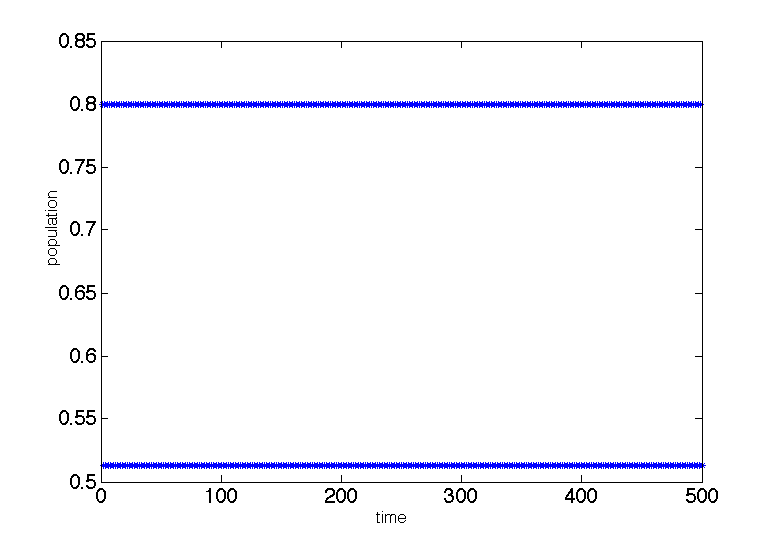
\includegraphics{figs/log_seq_32.png}

}

\subcaption{\label{fig-series}The steady state sequence of values
producef by iteration of the logistic map \(x_{n+1} = rx_n(1-x_n)\) for
\(r=3.2\)}

\end{minipage}%
%
\begin{minipage}{0.50\linewidth}

\centering{

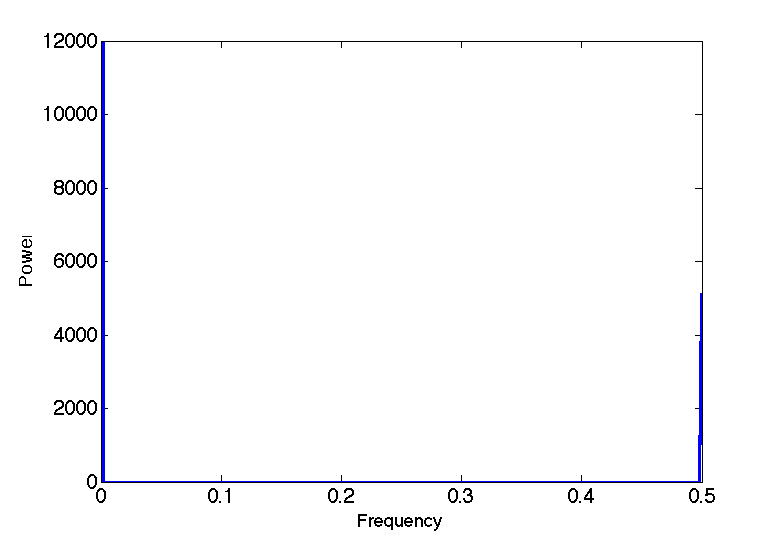
\includegraphics{figs/log_pow_32.png}

}

\subcaption{\label{fig-power}The power spectrum of the data produced by
iteration of the logistic map with \(r=3.2\)}

\end{minipage}%

\caption{\label{fig-log-map-32}Time series and power spectrum}

\end{figure}%

You can see that a period 2 oscillation is represented by two nonzero
values in the power spectrum: zero frequency (sum of all values) and
frequency 1/2 (period 2). This time of sharply peaked power spectrum is
expected from

Now let us take the value \(r=3.8\), which leads to chaotic behavior,
which is not periodic. The time series and the power spectrum are shown
below:

\begin{figure}

\begin{minipage}{0.50\linewidth}

\centering{

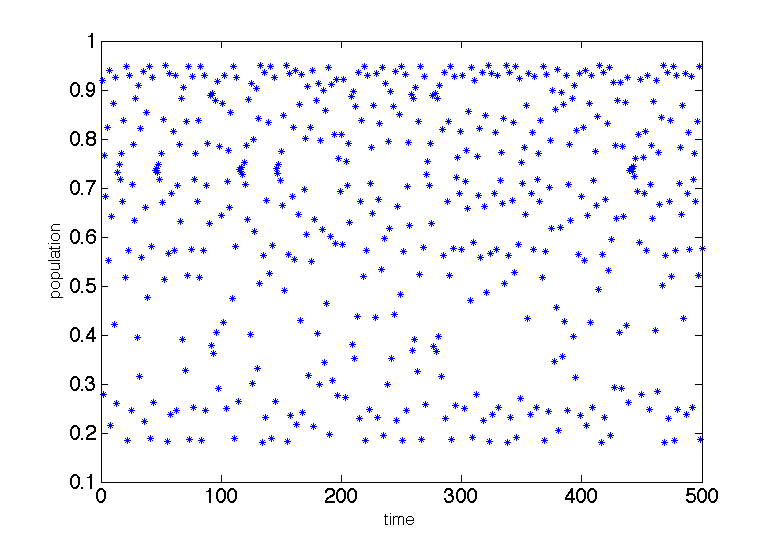
\includegraphics{figs/log_seq_38.png}

}

\subcaption{\label{fig-series}Sequence of values produced by iteration
of the logistic map \(x_{n+1} = rx_n(1-x_n)\) for \(r=3.8\)}

\end{minipage}%
%
\begin{minipage}{0.50\linewidth}

\centering{

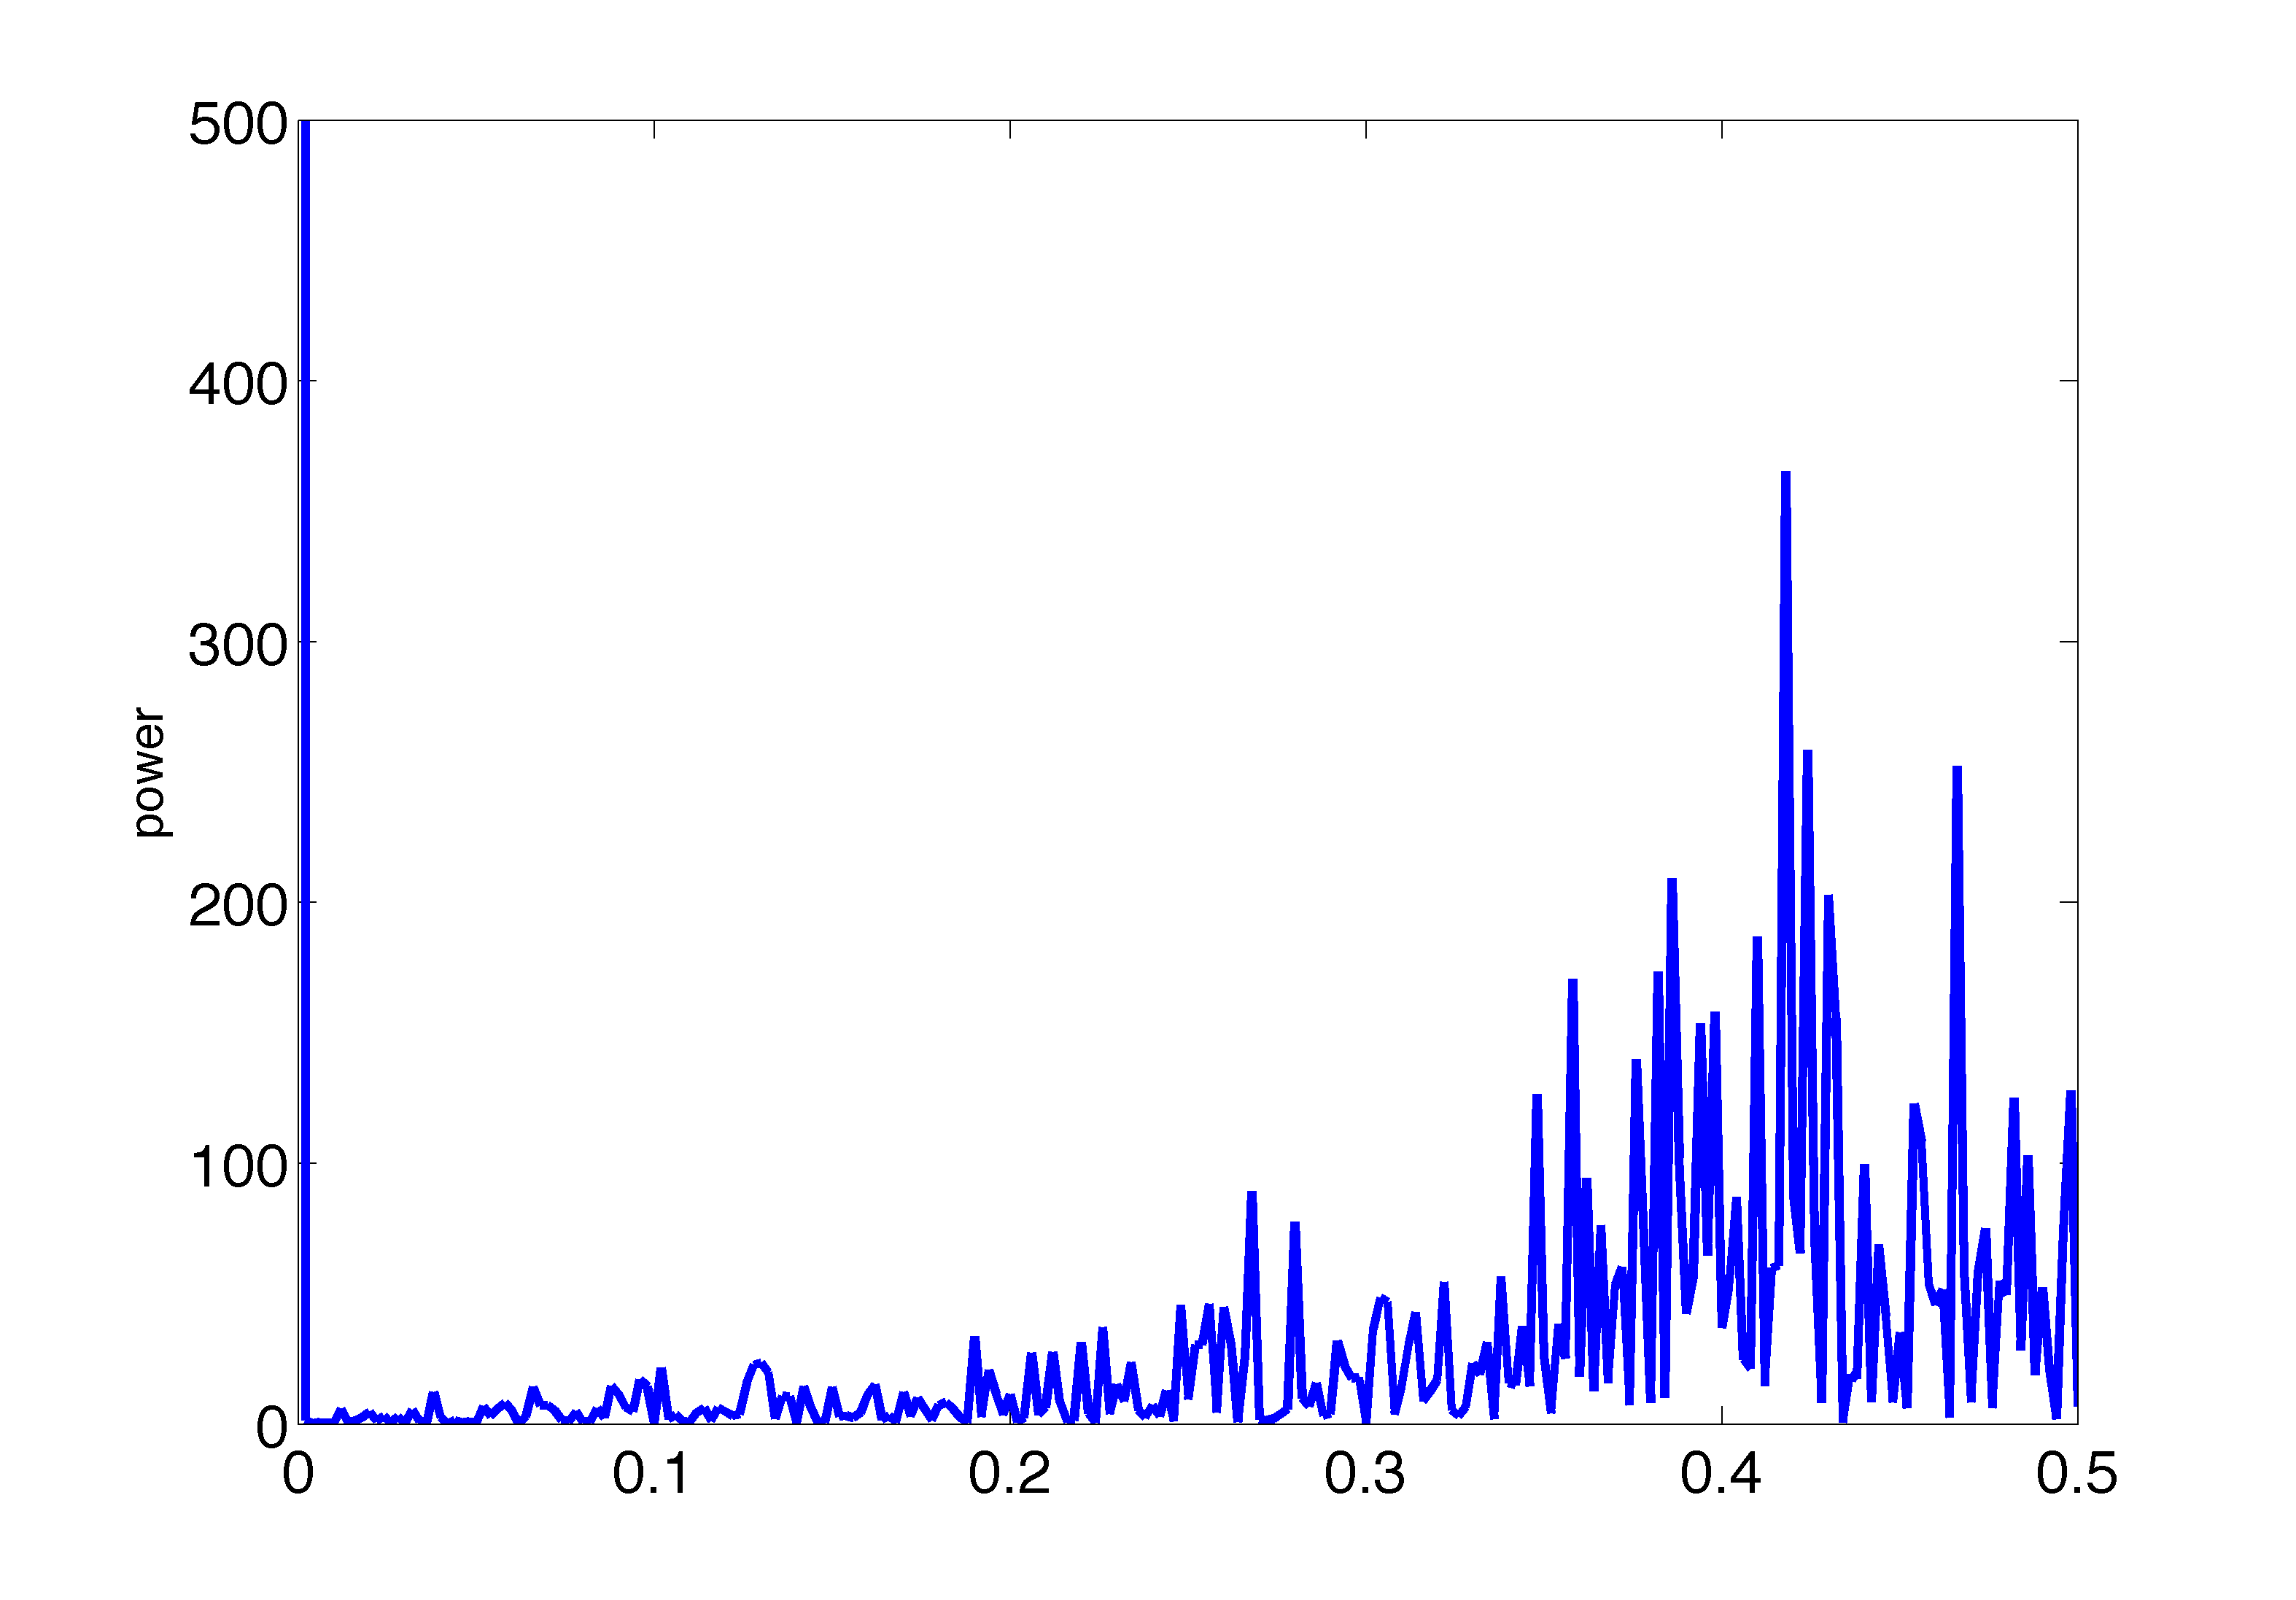
\includegraphics{figs/log_pow_38.png}

}

\subcaption{\label{fig-power}The power spectrum of the data produced by
iteration of the logistic map with \(r=3.8\)}

\end{minipage}%

\caption{\label{fig-log-map-38}Time series and power spectrum}

\end{figure}%

You can see that the power spectrum of a chaotic time series is
dramatically different: all frequencies contribute, fast and slow, but
the overall appearance of the power spectrum is ragged, as they are all
represented with different powers. This is a tell-tale mark of chaos:
lack of well-defined peaks, and an overall unstructured appearance.

\section{Synthesis: Fourier transform of crystal diffraction
pattern}\label{synthesis-fourier-transform-of-crystal-diffraction-pattern}

One important application of Fourier transforms is to optical
scattering. Any time light is scattered by an object, it results in a
Fourier transform of the image of the object, and if enough photons are
scattered, one can get a pretty complete picture. In the visible range,
we can use lenses, such as in our eyes or in microscopes, to essentially
perform the inverse Fourier transform. In X-ray crystallography, which
is the primary tool for determining structures of biological molecules
it is not possible, because no optical lenses can interact with photons
of that wavelength. We are left to perform the inverse Fourier
transforms computationally.

Each atom in the crystal scatters photons with its electron cloud. While
it is easy to describe the distribution of electrons in each atom, we
have many atoms arranged in a lattice, each contributing to the
diffraction intensity. If we consider them all, it will be a very
difficult calculation. Instead, the convolution property allows us to
find the Fourier transform of a single atom (a Gaussian function, so its
Fourier pair is another Gaussian) and find the transform of the
idealized lattice of points, both of which are easy calculations, and
then multiply them together to find the Fourier transform of the whole
lattice of atoms. This gives a simplified idea of how X-ray
crystallographers can make sense out of a diffraction pattern and
re-create the electron density inside the molecules in the crystal.

\bookmarksetup{startatroot}

\chapter{Discrete optimization problems: Monte Carlo
search}\label{discrete-optimization-problems-monte-carlo-search}

\section{Monte Carlo methods}\label{monte-carlo-methods}

Monte Carlo algorithms are used to find the optimal solution in a large
space of possible solutions, by randomly generating new candidates and
randomly deciding whether to accept or reject them. The stochastic
approach does not guarantee finding the global optimum, however, it
enables one to sample the space of possibilities, far outside of the
vicinity of the initial guess. Here is the outline of the method:

\begin{enumerate}
\def\labelenumi{\arabic{enumi}.}
\item
  Start with an initial guess \(\vec x_0\)
\item
  Generate a new candidate \(\vec x_{i+1}\), usually using a random
  algorithm. For example, given a path for the TSP, one can generate a
  new candidate path by swapping the order of two randomly chosen
  cities.
\item
  Evaluate the objecting function of the new candidate state and compare
  with the objective function at the old state. If the new candidate is
  better (\(f(\vec x_{i+1}) < f(\vec x_i)\)), accept the new state. If
  the new candidate does not have a lower objective function, use the
  \emph{Metropolis criterion} to randomly decide whether to accept the
  new state. Thus, if \(f(\vec x_{i+1}) > f(\vec x_i)\), accept the new
  state with probability \(P = e^{f(\vec x_{i-1}) - f(\vec x_i)}\).
\item
  Repeat until the algorithm no longer improves the objective function:
  usually, until a maximum number of consecutive rejections is reached.
\end{enumerate}

The fact that the Monte Carlo algorithm sometimes will accept a worse
(in term of the objective function) new candidate state means that it is
capable of climbing out of a local well which may not be the deepest.
This, of course, still does not guarantee that it finds the global
minimum in any finite amount of time. However, given enough iterations,
Monte Carlo can explore the space of possible states and find something
close to the global optimum.

\section{Traveling Salesman Problem}\label{traveling-salesman-problem}

We now proceed to complex optimization problems for which the objective
function either has no exact formula, or there is no way of computing
gradients and curvatures. One such class of cases are functions for
which the variables have only discrete domains. A famous example is the
\emph{traveling salesman problem}, in which the goal is to find the
optimal order of visiting \(N\) cities, with optimal meaning the order
with the lowest total distance traveled. This seemingly simple problem
has no efficient algorithm for solving it exactly - it belongs to a
class of problems known as ``NP-complete'' (I will not attempt to
explain the terminology here). All exact methods for solving the TSP are
as inefficient as the brute force method of considering every possible
order of visiting the cities, calculating the total distance of each,
and picking the best one. However, since the number of such paths is
\(N!\), this is an impractical way of solving the problem.

\section{Simple protein folding model: HP on a
lattice}\label{simple-protein-folding-model-hp-on-a-lattice}

Protein folding, as mentioned above, is a very complex problem of
finding the global energy minimum is a very large space of states. The
main driving force behind the process is the hydrophobic effect: the
preference of hydrophobic (oily) amino acid residues to stick together
and minimize their interactions with water. Some residues are
hydrophobic, and others are polar, and the latter usually end up in the
interior of a folded protein structure.

One extremely simple type of models to study the mechanism of protein
folding is the HP model on a lattice, where a protein is modeled as a
chain of beads, representing amino acid residues, each either
hydrophobic (H) or polar (P) in character. The positions of the beads
are restricted to a lattice, typically of cubic symmetry, so there are
only a discrete number of possible conformations, but just like in the
traveling salesman problem, they grow exponentially. To construct a
possible protein ``conformation'', one can start the chain at one end,
and then place the next bead in one of the neighboring lattice points
which not occupied. If one chooses the next step randomly, it is called
a ``self-avoiding random walk''.

The object is to find the conformation which minimizes the total energy.
Total energy is HP models can be defined differently, but the simplest
calculation is just to count the number of pairs of hydrophobic resides
which are neighbors (one lattice point away) and take the negative of
that number to be the total energy. Thus, there is a payoff for placing
hydrophobic residues near each other, and no effect from the location of
polar residues (which is not physically correct). You will use the
computer lab to explore this model using a Monte Carlo approach.

\bookmarksetup{startatroot}

\chapter{Markov models and transition
matrices}\label{markov-models-and-transition-matrices}

\section{Independence of random
variables}\label{independence-of-random-variables}

Two events are independent if: \(P(A\|B) = P(A)\). Since by definition
the conditional probability is \(P(A|B) = P(A\cap B)/P(B)\), the notion
of independence can be expressed as the \emph{product rule}, that states
that two events are independent if and only if:\[ 
P(A \cap B) = P(B)P(A)
\] Note that this allows us to shift the definition onto random
variables, since probability of a value \(x\) of a random variable \(X\)
corresponds to the probability of the event that gets mapped to \(x\).
Thus, the same definition applied to two random variables \(X\) and
\(Y\), in slightly different notation \[ 
P(X=x,Y=y) = P(X=x)P(Y=y)
\] for all values of \(x\) and \(y\).

\subsection{Example: strings of binary
trials}\label{example-strings-of-binary-trials}

The notion of independence is extremely useful for computing probability
of more complicated random variables. If we assume that Bernoulli trials
are independent of each other, then we can immediately calculate the
probability of a string of 0s and 1s or Ws and Ls given the probability
of a win is \(p\) and that of a loss is \(q\). For example:
\(P(\{WWLWL\}) = p^3q^2\).

In practice, independence between processes is rarely perfectly true.
However, computing the probability of two random variables without
independence is such a pain that it is often very useful to make the
independence assumption, and then test it against the data. If it stands
up, you have a good predictive model, and if it does not, you have
learned that two processes are somehow linked, which is very useful.

\section{Random variables that change with
time}\label{random-variables-that-change-with-time}

A \emph{stochastic process} is a sequence of random variables that
change with time. The changes may be in discrete time steps that can be
counted, and then we denote the random variable at time step \(n\)
\(X_n\). If time is continuous, not broken up into countable steps, then
there are infinitely many random variables \(X_t\) for any real number
\(t\). The random variables are assumed to all be functions with the
same domain (sample space), and with the same range (the numbers that
they can assume). What changes over time is the probability distribution
function of the random variables.

We already saw sequences of random variables in the case of repeated
Bernoulli trials. Those trials were independent of each other and each
random variable \(X_n\) had the same probability distribution. In (most)
other situations, the probability distribution at time \(n\) depends on
the distributions before, or the history of the stochastic process.

\subsection{Computing the probability one step
ahead}\label{computing-the-probability-one-step-ahead}

Let us say we know the probability distribution of \(X_n\), and we want
to know the probability distribution of \(X_{n+1}\). By the definition
of conditional probability,
\(P(X_{n+1} = x \; and \; X_n = y) = P(X_{n+1} =x | X_n = y) P(X_n = y)\).
Then, to find the total probability of \(X_{n+1} = x\), add up all the
probabilities \(P(X_{n+1} = x \; and \; X_n=y)\) for all possible values
of \(X_n\), since they add up to the whole sample space:

\[ 
P(X_{n+1} = x) = \sum _ {all \; y} P(X_{n+1} = x \; and \; X_n = y) = \sum _ {all \; y} P(X_{n+1} =x | X_n = y) P(X_n = y)
\]

Therefore, to compute the probability distribution of the next random
variable in time, we need to know the conditional probabilities of the
next random variable given the previous one. These are called
\emph{transition probabilities} and are the basis of the models we will
be studying.

\subsubsection{Example: weather changes}\label{example-weather-changes}

Suppose that the weather changes in a random way (big surprise), and we
divide it in only two states: sunny (\(S\)) and cloudy (\(C\)). Suppose
that the weather tomorrow \(W_{n+1}\) depends on the weather today
\(W_n\) with the following transition probabilities (perhaps obtained
empirically over years of observations) given in the table below.

\begin{longtable}[]{@{}lll@{}}
\toprule\noalign{}
& sunny today & cloudy today \\
\midrule\noalign{}
\endhead
\bottomrule\noalign{}
\endlastfoot
sunny tomorrow & 0.8 & 0.3 \\
cloudy tomorrow & 0.2 & 0.7 \\
\end{longtable}

Given these conditional probabilities, we can compute the probability
distribution of the weather tomorrow given the weather today, e.g., if
today is sunny, then the probability it will be sunny tomorrow is
\(P(W_{n+1} = S ) =\)
\[ = P(W_{n+1} = S | W_n = S) P(W_n = S) + P(W_{n+1} = S | W_n = C) P(W_n = C) = 0.8 * 1  + 0.3* 0 = 0.8\]
Similarly \(P(W_{n+1} = C)=\)
\[ = P(W_{n+1} = C | W_n = S) P(W_n = S) + P(W_{n+1} = C | W_n = C) P(W_n = C) = 0.2 * 1  + 0.7* 0 = 0.2\]

We can go further and compute the probability of the weather two days
into the future, by applying the transition probabilities again:
\(P(W\_{n+2} = S ) =\)
\[P(W_{n+2} = S | W_{n+1} = S) P(W_{n+1} = S) + P(W_{n+2} = S | W_{n+1} = C) P(W_{n+1} = C) = 0.8 * 0.8  + 0.3* 0.2 = 0.7\]
and also \(P(W_{n+2} = C) =\)
\[P(W_{n+2} = C | W_{n+1} = S) P(W_{n+1} = S) + P(W_{n+2} = C | W_{n+1} = C) P(W_{n+1} = C) = 0.2 *0.8  + 0.7* 0.2 = 0.3\]

These calculations could be written more succinctly as a product of a
\emph{transition matrix} \(M\) and the vector with the probability
distribution. The probabilities for next day's weather given sunny
weather today are: \[  
\left(\begin{array}{cc}0.8& 0.3 \\0.2 & 0.7\end{array}\right)   \left(\begin{array}{c}1\\0 \end{array}\right) =  \left(\begin{array}{c} 0.8\\0.2\end{array}\right)  
\] And the probabilities for the next day are computed by multiplying by
the matrix again. So it can be written as multiplying the first
probability distribution by the square of the transition matrix:

\[ 
\left(\begin{array}{cc}0.8& 0.3 \\0.2 & 0.7\end{array}\right) \left(\begin{array}{c}0.8\\0.2 \end{array}\right) =   \left(\begin{array}{cc}0.8& 0.3 \\0.2 & 0.7\end{array}\right)  \left(\begin{array}{cc}0.8& 0.3 \\0.2 & 0.7\end{array}\right)  \left(\begin{array}{c}1\\0 \end{array}\right) =  \left(\begin{array}{cc}0.8& 0.3 \\0.2 & 0.7\end{array}\right) ^2  \left(\begin{array}{c}1\\0 \end{array}\right) = \left(\begin{array}{c} 0.7\\0.3\end{array}\right) 
\] We can multiply the initial distribution by the transition matrix
\(n\) times obtain the probability distribution for weather \(n\) days
in the future.

\section{Markov chains}\label{markov-chains}

The above is an example of generating a sequence of probability
distributions for random variables known as a \emph{Markov chain}. The
random variables must have a finite number of possible values (known as
states) so the probability distributions can be written as vectors
\(P_n\), and the transition matrix \(M\) where each element \(\pi_{ij}\)
(in the \(i\)-th row and the \(j\)-th column) is known as a
\emph{transition probability} \(P(X_{n+1} = x_i | X_n = x_j)\), where
\(x_i\) and \(x_j\) are the \(i\)-th and the \(j\)-th state of the
random variable \(X_n\). Then, as we saw above, the probability
distribution at time \(n\) is given by:

\[ 
P_{n+1} = MP_n \; \Longrightarrow P_{n} = M^nP_0
\]

where \(P_0\) is initial probability distribution.

What makes such a stochastic process \emph{Markovian} is a deep
assumption which is implicit in our definition. We assumed that we can
calculate the probability distribution of the variable at the next time
knowing only the distribution at the present time. More precisely, we
assumed that \textbf{the conditional probability distribution at time}
\(n+1\), given the random variable at time \(n\), is \emph{independent}
of the knowledge of the random variable at time \(n-1\) or any previous
time.

This is called the \emph{Markov property}, and it can be written as
follows: \[
P(X_{n+1} | X_{n} , X_{m}) = P(X_{n+1} | X_{n}),  \; for \;  m<n 
\]

\subsection{properties of Markov transition
matrices}\label{properties-of-markov-transition-matrices}

The transition matrices, a.k.a. Markov matrices, have some special
properties that help us compute the Markov chain they generate:

\begin{itemize}
\tightlist
\item
  By construction each column of a Markov matrix (with \(m\) states) has
  to add up to 1, because \[
  \sum_{i=1}^{m} \pi_{ij} = \sum_{i=1}^{m} P(X_{n+1} = x_i | X_n = x_j) = 1
  \] since all possible outcomes have to add up to 1.
\item
  Multiplying a probability distribution vector by a Markov matrix
  preserves the property that all elements add up to 1 (check for
  yourself that this follows from the first property.)
\item
  The eigenvalues of the Markov matrix are all \(|\lambda | <1\). This
  is important because to calculate powers of the matrix, we can use the
  diagonal form \(M = U \Lambda U^{-1}\) where \(U\) is the matrix of
  eigenvectors and \(\Lambda\) is the matrix of eigenvalues; then
  \(M^n = U \Lambda^n U^{-1}\). Therefore, each eigenvalue is raised to
  the \(n\)-th power, and given the property above, all the eigenvalues
  except for \(\lambda =1\) will decay. Those eigenvectors with
  eigenvalue unity are called \emph{stationary probability
  distributions}.
\item
  The elements of \(M\) are probabilities and therefore are between 0
  and 1, inclusively. If all the elements are strictly greater than zero
  (and thus strictly less than 1), there is only a single eigenvalue
  equal to 1 and thus only a single equilibrium probability
  distribution.
\end{itemize}

\subsection{Example: Hardy-Weinberg
equilibrium}\label{example-hardy-weinberg-equilibrium}

Here is an application of the concept of an equilibrium distribution,
known as the Hardy-Weinberg equilibrium. This is a classic population
genetics result for the distribution of frequencies of genotypes in a
population. We assume that the population consists of randomly mating
diploid individuals, and that we are only interested in two alleles of a
gene: \(A\) and \(a\). For a diploid individual, there are three
possible genotypes: \(AA\), \(aa\), and \(Aa\) (same as \(aA\)). The
frequencies of these genotypes in the population are equivalent to the
probabilities of a given individual possessing that genotype. Let us
call the initial frequencies as follows: \(P_0(AA) = p_0\),
\(P_0(aa) = q_0\), \(P_0(Aa) = r_0\).

The conditional probability of inheriting one \(A\) allele given one
parent has \(AA\) is \(P (A | AA) = 1\), similarly \(P(A | aa) = 0\),
and \(P(A | Aa) = 1/2\). Then we can calculate the total probability of
inheriting an allele in the next generation is:
\[ P(A) = P (A | AA)p_0 + P(A | aa) q_0 + P(A | Aa) r_0 = p_0 + r_0/2\]

\[ P(a) = P (A | AA)p_0 + P(A | aa) q_0 + P(A | Aa) r_0 = q_0 + r_0/2\]

The probability of having the genotype \(AA\) is the product of the two
probabilities, because of the independence assumption in random mating.
Thus we obtain the frequencies of the three genotypes in the next
generation:

\[P(AA) = P(A) P(A) = (p_0 + r_0/2)^2 = p_1\]

\[P(aa) = P(a) P(a) = (q_0 + r_0/2)^2 = q_1\]
\[P(Aa) = P(A) P(a) + P(a)P(A) = 2(q_0 + r_0/2)(p_0 + r_0/2) = r_1\]

The transition matrix can be written by assuming the transition
probabilities \(P(AA | AA) = p + r/2\) (probability of offspring with
genotype \(AA\), given that one parent has genotype \(AA\), is the
probability of finding allele \(A\) in the population). Similarly,
\(P(aa | aa) = q + r/2\), \(P(Aa | AA) = q + r/2\), and
\(P(Aa | aa) = p + r/2\). Of course, \(P(aa | AA ) = P(AA | aa) = 0\).
If the parent is heterozygous, then the conditional probability is
\(P(AA | Aa) = 1/2( p + r/2)\), the product of the frequency of the
allele \(A\) and the probability of \(A\) being passed on from the
heterozygote (1/2). Similarly, \(P(aa | Aa ) = 1/2( q + r/2)\). Finally,
the most complicated transition probability
\(P(Aa | Aa) = P(A) 1/2 + P(a) 1/2 = p/2 + r/2 + q/2\). The transition
matrix is then:
\[ M = \left(\begin{array}{ccc}p + r/2 & 0 & p/2 + r/4 \\0 & q + r/2 & q/2 + r/4 \\ q + r/2 &  p + r/2 & p/2 + q/2 + r/2\end{array}\right) \]

Here we can find the equilibrium distribution by requiring that
\(M P_s = P_s\), which is equivalent to the following equations:

\[ p = p (p + r/2) + r (p/2 + r/4) = (p + r/2)^2\]
\[ q = q(q + r/2) + r (q/2 + r/4) = (q + r/2)^2 \]
\[ r = p(q + r/2) + q(p+r/2) + r (p/2 + q/2 + r/2) = 2(p + r/2)(q + r/2) \]
Check that the three frequencies add up to 1, as they are supposed to.
Note that these are the same expressions we derived above for the
frequency distribution after 1 generation, only now the frequencies
\(p\), \(q\), and \(r\) are the same on both sides. These are the
conditions for the Hardy-Weinberg equilibrium in a randomly mating
population with no selection.

\subsection{Example: models of base substitution in
DNA}\label{example-models-of-base-substitution-in-dna}

The following is a summary of the material from Chapter 4 of Allman \&
Rhodes, \emph{Mathematical Models for Biology}. Substitution mutations
in DNA sequences can be modeled as a Markov process, where each base in
the sequence mutates independently of others with a transition matrix
\(M\). Let the bases A, G, C, T correspond to states 1 through 4,
respectively. One possible model for base substitution from one
generation to the next is based on the assumption that all substitution
mutations are equally likely, and that the fraction \(\alpha\) of the
sequence will be substituted each generation. Then the probability of
any particular transition, say from T to C is \(\alpha/3\), while the
probability of not having a substitution is equal to \(1-\alpha\). This
is known as the Jukes-Cantor model and it predicts that the fraction of
letters in a sequence at generation \(t+1\) depends on the distribution
in generation \(t\) as follows:

\[   
\left(\begin{array}{c} P_A \\ P_G \\ P_C \\ P_T \end{array}\right)_{t+1}  = \left(\begin{array}{cccc}1-\alpha & \alpha/3 & \alpha/3 & \alpha/3 \\\alpha/3 & 1-\alpha & \alpha/3 & \alpha/3 \\\alpha/3 & \alpha/3 & 1-\alpha & \alpha/3 \\\alpha/3 & \alpha/3 & \alpha/3 & 1-\alpha\end{array}\right) \left(\begin{array}{c} P_A \\ P_G \\ P_C \\ P_T \end{array}\right)_t 
\]

This model is very simple: it only considers substitutions, although
other mutations are possible, e.g.~insertions and deletions, although
they are typically more disruptive and thus more rare, and it treats all
substitutions as equally likely, which is not empirically true. The
benefit is that the number \(\alpha\) is the only parameter in this
model, which represents the mutation rate at each site per generation.
This makes is easy to compute the eigenvectors and eigenvalues of the
model in general. It turns out that the four eigenvectors do not depend
on the parameter \(\alpha\), only the eigenvalues do:

\[  
\left(\begin{array}{c} 1/4 \\ 1/4 \\ 1/4 \\ 1/4 \end{array}\right) \lambda =1; \; \left(\begin{array}{c} 1/4 \\ -1/4 \\ 1/4 \\ -1/4 \end{array}\right)\lambda =1-4/3\alpha;  \; \left(\begin{array}{c} 1/4 \\ -1/4 \\ -1/4 \\ 1/4 \end{array}\right)\lambda =1-4/3\alpha;  \; \left(\begin{array}{c} 1/4 \\ -1/4 \\ 1/4 \\ -1/4 \end{array}\right)\lambda =1-4/3\alpha 
\]

Notice two things: first, the first eigenvector is the equilibrium
distribution and has the same frequencies for all four bases. Second,
the three eigenvectors with eigenvalues smaller than 1 have negative
entries, so they cannot be probability distributions themselves
(although as linear combinations with the first one, they may be,
depending on the coefficients.) A computational sidenote: because the
three non-equilbrium eigenvectors share the same eigenvalue, it is
possible to choose multiple valid sets of eigenvectors. For instance,
MATLAB returns different answers for the eigenvectors above. This is
because of non-uniqueness of eigenvectors that share the same eigenvalue
(a topic which we have avoided in this course, but is covered in linear
algebra textbooks.)

Computationally, this allows us to predict the time evolution of a
distribution of bases in a DNA sequence for any given initial
distribution, by using repeated matrix multiplication as above. Figure
below shows the results starting with a non-equilibrium base
distribution for 20 generations, with different substitution rates. It
is evident that for a faster substitution rate the approach to the
equilibrium distribution is faster. This demonstrates an important role
of the second-largest eigenvalue of the Markov matrix: it determines the
speed of convergence to the equilibrium distribution (more on this
later).

\{\#fig-JC-model layout-ncol=2\}

\begin{figure}[H]

{\centering 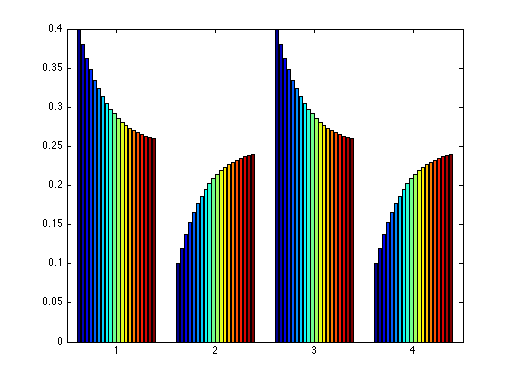
\includegraphics{figs/base_sub_01.png}

}

\caption{\(\alpha = 0.1\)}

\end{figure}%%
\begin{figure}[H]

{\centering 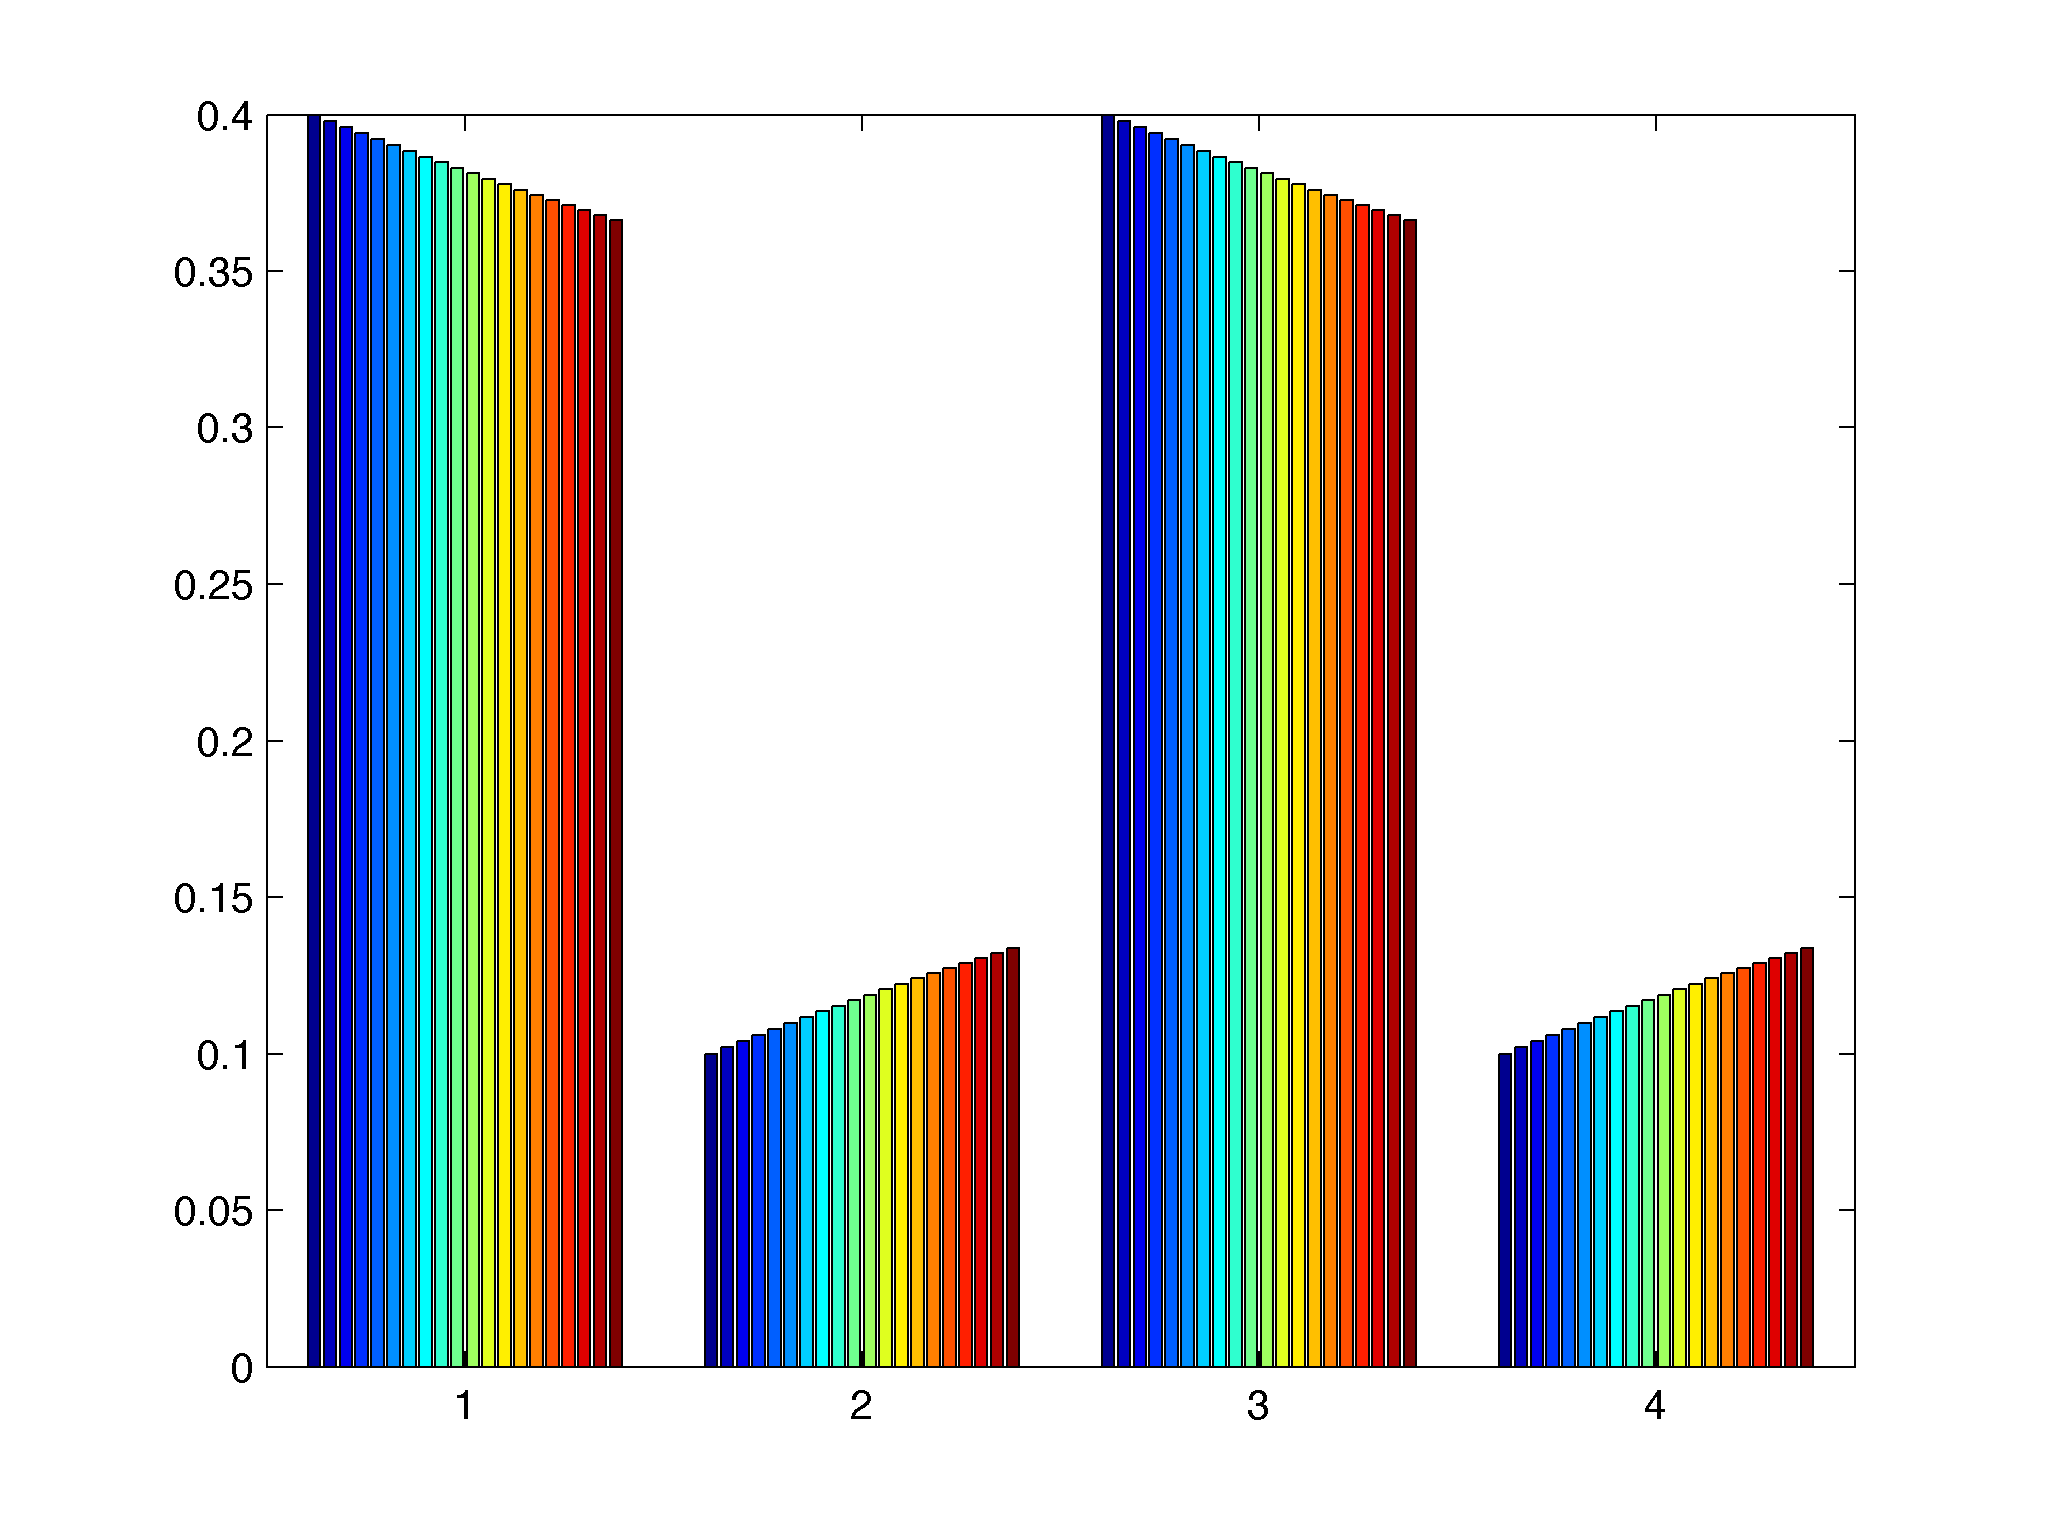
\includegraphics{figs/base_sub_001.png}

}

\caption{\(\alpha = 0.01\)}

\end{figure}%

Evolution of base distribution for different substitution rates, with
bar graphs showing proportion of letters A, G, T, C from generation 0 to
20 :::

\subsubsection{calculation of phylogenetic
distances\}}\label{calculation-of-phylogenetic-distances}

As we saw, the Markov model provides a means of measuring the
time-dependent evolution of the probability distribution of each letter,
starting with some initial distribution. In reality, we would like to
answer the following question: given two DNA sequences in the present
(e.g.~from different species), what is the length of time they spent
evolving from a common ancestor?

To do this, we need to some preliminary work. The first step is to
compute the probability that a letter at a particular site remain
unchanged after \(t\) generations. Because all the nucleotides are
equivalent in the Jukes-Cantor model, we need to find
\(P(X_t = A | X_0 = A)\). More generally, we can calculate the frequency
distribution after \(t\) time steps as follows: \(P_t = M^t P_0\). In
this case, \(P_0 = (1,0,0,0)\), which can be written as a sum of the
four eigenvectors of the matrix \(M\):

\[ 
\left(\begin{array}{c} 1 \\ 0 \\ 0 \\ 0 \end{array}\right) = \left(\begin{array}{c} 1/4 \\ 1/4 \\ 1/4 \\ 1/4 \end{array}\right) + \left(\begin{array}{c} 1/4 \\ -1/4 \\ 1/4 \\ -1/4 \end{array}\right) +  \left(\begin{array}{c} 1/4 \\ -1/4 \\ -1/4 \\ 1/4 \end{array}\right) + \left(\begin{array}{c} 1/4 \\ -1/4 \\ 1/4 \\ -1/4 \end{array}\right) 
\]

Therefore, the matrix \(M^t\) can be applied to each eigenvector
separately, and each matrix multiplication is a multiplication by the
appropriate eigenvalue. Thus,

\[ 
P_t = M^t P_0 =   1^t \left(\begin{array}{c} 1/4 \\ 1/4 \\ 1/4 \\ 1/4 \end{array}\right) + (1-\frac{4}{3}\alpha)^t\left( \left(\begin{array}{c} 1/4 \\ -1/4 \\ 1/4 \\ -1/4 \end{array}\right) +  \left(\begin{array}{c} 1/4 \\ -1/4 \\ -1/4 \\ 1/4 \end{array}\right) + \left(\begin{array}{c} 1/4 \\ -1/4 \\ 1/4 \\ -1/4 \end{array}\right) \right)
\]

The first element of \(P_t\) is the probability of a nucleotide
remaining \(A\) after \(t\) generation, and it is:

\[
P_t(A) = \frac{1}{4} + \frac{3}{4}\left(1-\frac{4}{3}\alpha\right)^t
\]

For \(t=0\), the probability is 1, as it should be, and as
\(t \rightarrow \infty\), \(P_t(A) \rightarrow 1/4\), since this is the
equilibrium probability distribution. Note that the expression is the
same for all the other letters, so we have found the expression for any
nucleotide remaining the same after \(t\) generations.

Now let us get to the question of calculating the time that two
sequences have evolved from each other. Denote by \(m\) the fraction of
sites in two aligned sequences with different letters, and \(q\) is the
probability of a nucleotide remaining the same, which is the given by
the expression for \(P_t(A)\). Thus

\[
m = 1 - q = \frac{3}{4} - \frac{3}{4}\left(1-\frac{4}{3}\alpha\right)^t
\].

This can be solved for \(t\):

\[ 
t = \frac{\log (1 - \frac{4}{3}m)}{\log (1 - \frac{4}{3} \alpha)}
\]

However, we do not necessarily know the mutation rate \(\alpha\), so
this formula is mainly of theoretical interest. Instead, we would like
to calculate the \emph{phylogenetic distance} between the two sequences,
which is defined as \(d = \alpha t\), or the mean number of
substitutions that occurred per nucleotide during \(t\) generations,
with mutation rate \(\alpha\) (substitutions per nucleotide per
generation). Note that this distance is not directly measurable from the
fraction of different nucleotides in the two sequences, because it
counts all substitutions, including those which reverse an earlier
mutation, and cause the sequence to revert to its initial letter.

Now, let us assume \(\alpha\) is small, as typically the number of
substitutions per generation per nucleotide is small. Then, by a Taylor
expansion of the logarithm around 1,
\(\log (1 -\frac{4}{3} \alpha) \approx - \frac{4}{3}\alpha\). Using the
formula for \(t\) from above with this approximation, we find the
Jukes-Cantor phylogenetic distance to be:

\[ 
d_{JC} = \frac{\log (1 - \frac{4}{3}m)}{ - \frac{4}{3} \alpha} \alpha =  -\frac{3}{4}\log (1 - \frac{4}{3} m)
\]

This formula has the correct behavior in the two limits: when \(m = 0\),
\(d_{JC} = 0\) (identical sequences have zero distance), and when
\(m \rightarrow 3/4\), \(d_{JC} \rightarrow \infty\), since 3/4 is the
maximum possible fraction of differences under the Jukes-Cantor model.
Thus, we have obtained an analytic formula for the phylogenetic distance
based on a Markov chain model of substitutions.

\subsection{Kimura model}\label{kimura-model}

One can devise more sophisticated models of base substitution. There are
two classes of nucleotide bases: purines (A,G) and pyrimidines (C,T).
One may consider the difference in rates of \emph{transitions}
(substitutions within the classes) and \emph{transversions}
(subtitutions of purines by pyrimidines and vice versa). This is known
as the Kimura model and can be written as follows as Markov chain:

\[   
\left(\begin{array}{c} P_A \\ P_G \\ P_C \\ P_T \end{array}\right)_{t+1}  = \left(\begin{array}{cccc}1-\beta-\gamma & \beta & \gamma/2 &  \gamma/2 \\ \beta  & 1-\beta-\gamma & \gamma/2 & \gamma/2 \\ \gamma/2 & \gamma/2 & 1-\beta-\gamma& \beta  \\ \gamma/2 &\gamma/2 & \beta  & 1-\beta-\gamma \end{array}\right) \left(\begin{array}{c} P_A \\ P_G \\ P_C \\ P_T \end{array}\right)_t 
\]

where \(\beta\) is the rate of transitions and \(\gamma\) is the rate of
transversions per generation. This model has two different parameters,
and as those two rates are empirically different (transitions occur more
frequently, since the bases are more chemically similar,) the model is
more realistic. Whether or not it is worth the additional complexity
depends on the question at hand.

\subsection{Example: genetic drift as Bernoulli
trials}\label{example-genetic-drift-as-bernoulli-trials}

Now we come to another model of genetic variation in a population.
Consider a population of \(N\) haploid individuals with two genotypes
\(A\) and \(a\). Suppose that there are \(k\) individuals with allele
\(A\) (and therefore \(N-k\) individuals with allele \(a\)). Let the
population stay constant at \(N\), and assume that each individual has
an equal chance of passing on its allele to the next generation. It
follows that any given offspring inherits the allele \(A\) with
probability \(p = k/N\), and inherits allele \(a\) with probability
\(1-p = (N-k)/N\). Then generating the next generation of \(N\)
individuals is equivalent to \(N\) Bernoulli trials (coin tosses) with
those probabilities. Let the random variable \(X_t\) stand for the
number of individuals with allele \(A\) in generation \(t\). Then

\[
P(X_{t+1} = j | X_t = k) = C^N_j p^j (1-p)^{N-j} = \frac{N!}{j! (N-j)!} \left(\frac{N}{k}\right)^j \left(\frac{N-k}{k}\right)^{N-j}
\]

This defines the transition probabilities of an \(N\)-state Markov
chain. The probabilities of having \(j\) individuals with allele \(A\)
can be computed solely from the probability distribution in the previous
generation. These transition probabilities are dependent only on the
values of respective states \(j\) and \(k\), and the population size
\(N\), so the transition matrix is constant through the generations.

Note that there are two states from which there is no escape:
\(X_t = 0\) (all \(a\)) and \(X_t = N\) (all \(A\)). Since we did not
account for mutation, if a population randomly drifts to either of the
two states, it will remain there. This is known as \emph{fixation} of
the allele \(a\) or \(A\) in the population.

\bookmarksetup{startatroot}

\chapter*{References}\label{references}
\addcontentsline{toc}{chapter}{References}

\markboth{References}{References}

\phantomsection\label{refs}
\begin{CSLReferences}{0}{1}
\end{CSLReferences}



\end{document}
